\documentclass[12pt]{article}

\usepackage[scale=0.87]{geometry}
\usepackage{pdfpages}
\usepackage{tabularx}
\begin{document}

\begin{titlepage}
    \vspace*{\fill}
    \begin{center}
        \section*{Events in Language and Cognition - 2016}
    \end{center}
    \vspace*{\fill}
\end{titlepage}
\newpage

\section*{Organizers}

Eva Wittenberg, UC San Diego  \\
Melissa Kline, MIT \\
Joshua Hartshorne, Boston College 

\section*{Program Committee}

Ben Ambridge,
Curt Anderson,
Ryan Blything,
Peter Culicover,
Annelot de Rechteren van Hemert,
Monique Flecken,
Nate George,
Tilbe Goksun,
Roberta Golinkoff,
Angela He,
Anita Krishnan,
Laura Lakusta,
Kyle Mahowald,
Titus von der Malsburg,
Emily Morgan,
Mark Myslin,
Ken Nakatami,
Laura Niemi,
Liuba Papeo,
Shannon Pruden,
Jason Rothman,
Elliot Saltzman,
David Townsend,
Ercenur Unal.

\section*{Helpers}
Edith Kaan, Marc Matthews, Suhas Arehalli, Michelle Waters, George Collins

\newpage
\section*{Workshop Description}

Understanding how speakers wrap event conceptualizations into linguistic descriptions is crucial for both linguistic theory and psychology. A number of rich linguistic theories have been proposed to account for the observed ways that meaning maps to syntax within and across languages, but their psychological status remains unclear. These theories often propose specific representational architecture, ranging from prototype theories to predicate decomposition. How are these conceptual models and mappings grounded in non­linguistic cognition? On the side of cognitive science, our understanding of event representation, especially in infancy, has advanced dramatically in the past several decades, potentially opening up new possibilities for evaluating the plausibility of proposed argument structure theories. What can the understanding of event perception and cognition teach us about the nature of semantic representations for language, and how can psycholinguistic evidence contribute to research on event structure?

We aim to bring together psycholinguists interested in how language maps onto event structure, adding momentum to a growing field of interdisciplinary scholarship of event representation in linguistics, psycholinguistics, and cognitive science. We define three broad questions of interest:

(1) How do children and adults mentally represent events at the level of abstraction that is encoded in language?

(2) How is the structure of events represented in and conveyed by language?

(3) How to the constraints of the infant cognitive system and questions of learnability constrain our theories of language – and how does language constrain our theories of the infant cognitive system?

Several fields are currently approaching each of these questions, though with different theoretical underpinnings, methods, and terminologies. Given that, what should we be working on as an interdisciplinary field? Are there specific empirical questions that would be relevant to all theoretical perspectives? And what is necessary in order to bring together psycholinguists working on different questions? In this workshop, we want to both foster an exchange of recent work, and set a possible agenda for psycholinguistic research on event structure as conveyed by language.

\newpage
\section*{Workshop Schedule}
\begin{table}[h]
\begin{tabularx}{\textwidth}{r X}
    8:30 & Welcome, poster previews \\
    9:00 & \textbf{Elsi Kaiser}, Keynote Speaker \\
    9:45 & \textbf{Gerwien \& von Stutterheim} \\
         & \textit{Grammatical constraints on event packaging and potential effects on the segmentation of the perceptual stream.} \\
   10:15 & \textbf{Lundquist, Corley, Ramchand, Sorace, \& Tungseth} \\
         & \textit{Crosslinguistic variation in event conceptualization: Evidence from the causative alternation.}\\
   10:45 & Break \\
   11:15 & \textbf{Colicover, Alishahi, \& Vaiksnoraite} \\
         & \textit{The constructional evolution of grammatical functions and the thematic representation of events.}\\
   12:15 & \textbf{Altmann} \\
         & \textit{Multiple object-states represent events: A new account of event representation.} \\
   12:45 & Lunch Break \\
    1:45 & \textbf{Jesse Snedeker}, Keynote Speaker\\
    2:30 & \textbf{Foppolo, Panzeri, Greco, \& Carminatti} \\
         & \textit{The incremental processing of accomplishment predicates.} \\
    3:00 & \textbf{Venhuizen, Brouwer, \& Crocker} \\
         & \textit{When the food arrives before the menu: Modeling event-driven surprisal in language comprehension.} \\
    3:30 & Break \\
    3:45 & Poster Session \\
    4:45 & \textbf{Jeremy Skipper \& Elliot Saltzmann} (With Kaiser and Snedeker) \\
         & Panel Discussion \\
\end{tabularx}
\end{table}

\newpage
    \vspace*{\fill}
    \begin{center}
        \section*{Abstracts}
    \end{center}
    \vspace*{\fill}
\newpage

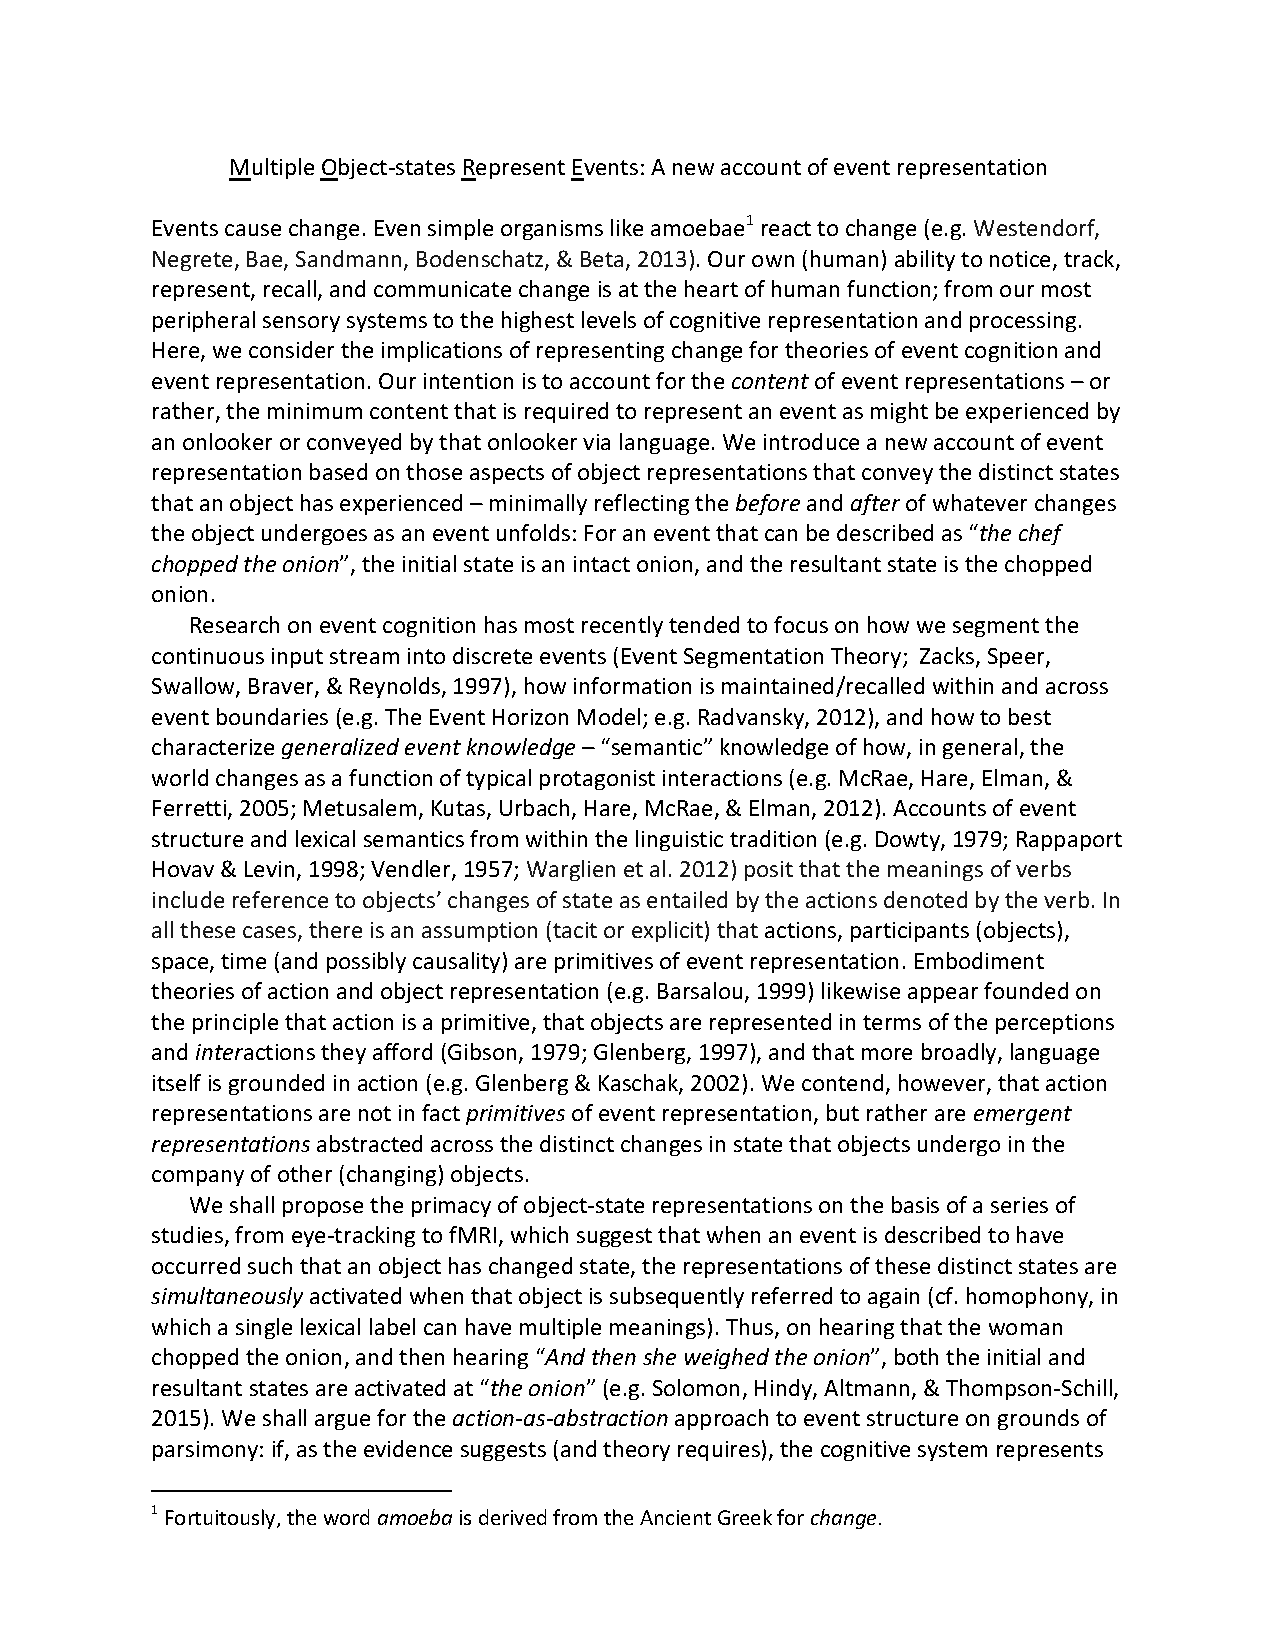
\includepdf[pagecommand={\thispagestyle{plain}}, pages=-]{01_ELC2016_paper_29.pdf}
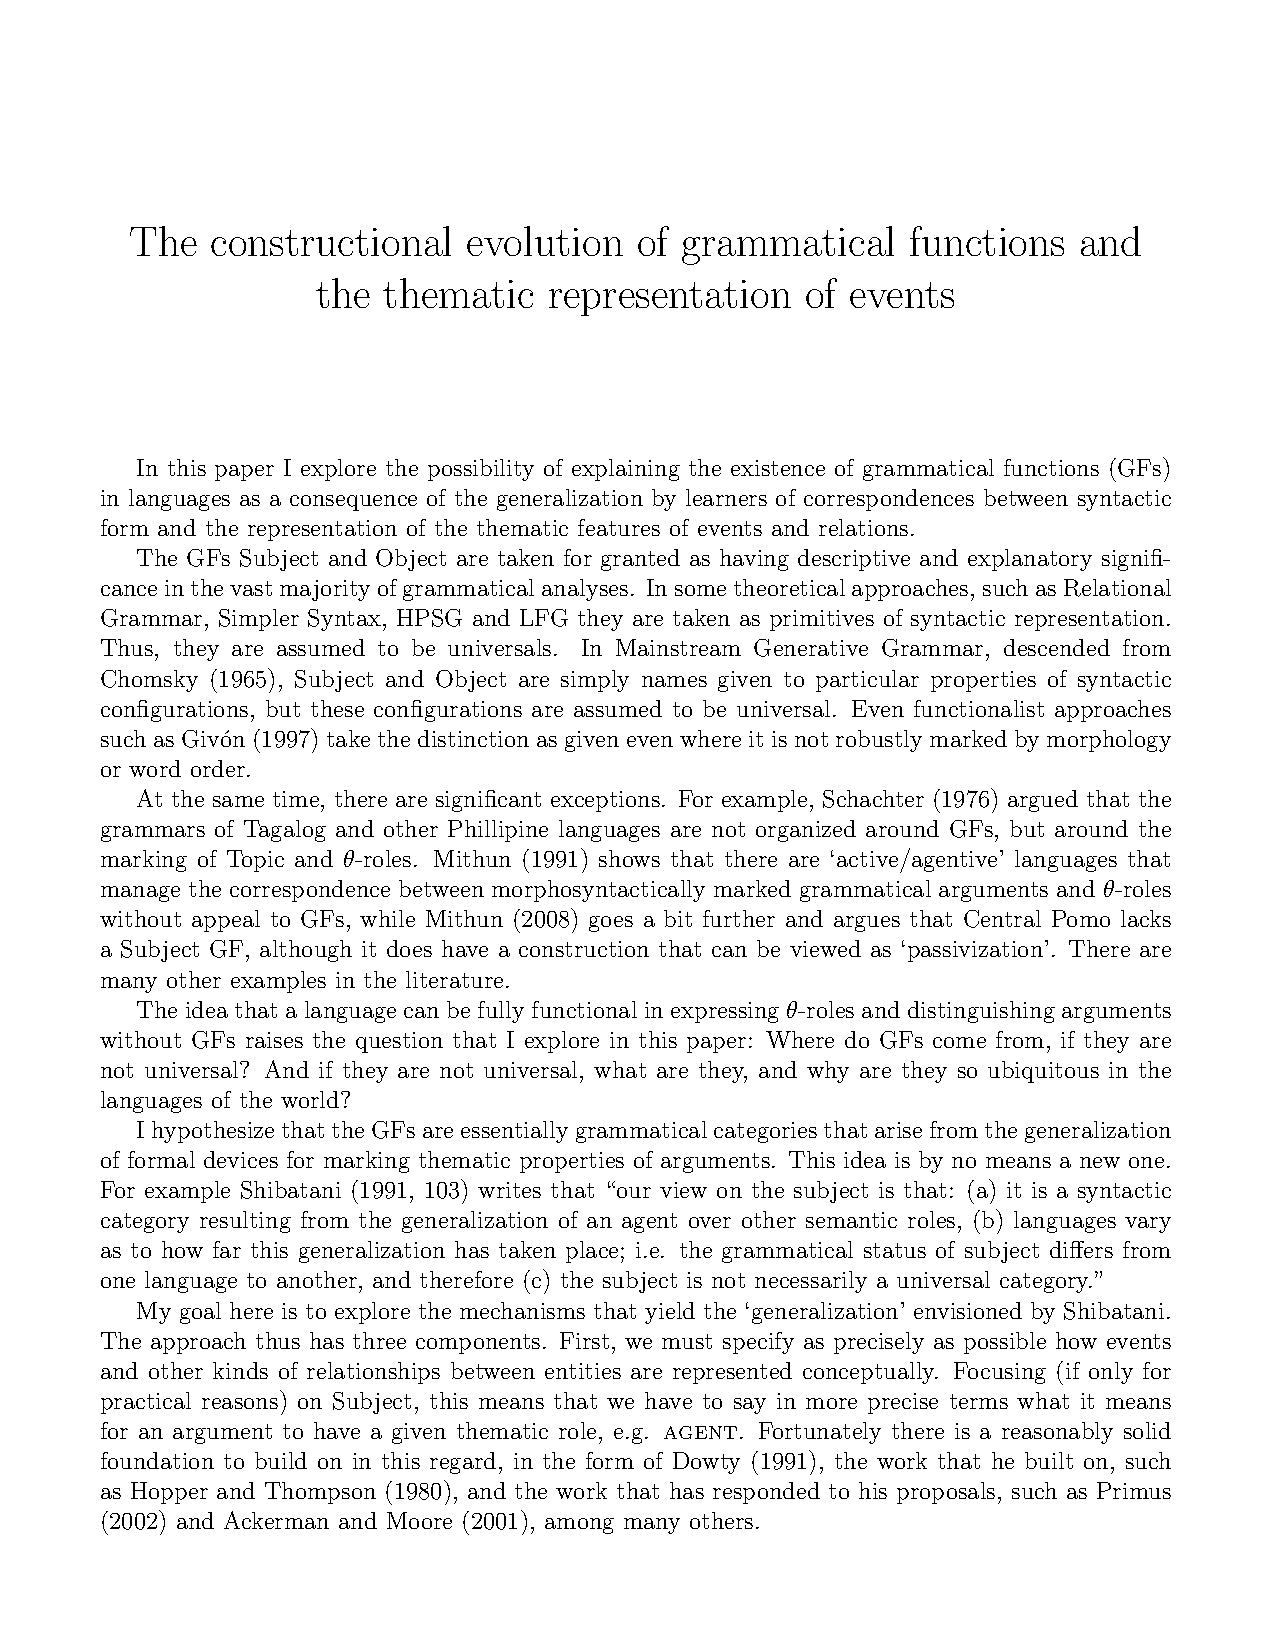
\includepdf[pagecommand={\thispagestyle{plain}}, pages=-]{02_ELC2016_paper_7.pdf}
\includepdf[pagecommand={\thispagestyle{plain}}, pages=-]{"02_The constructional evolution of grammatical functions and the representation of events (abstract) v2".pdf}
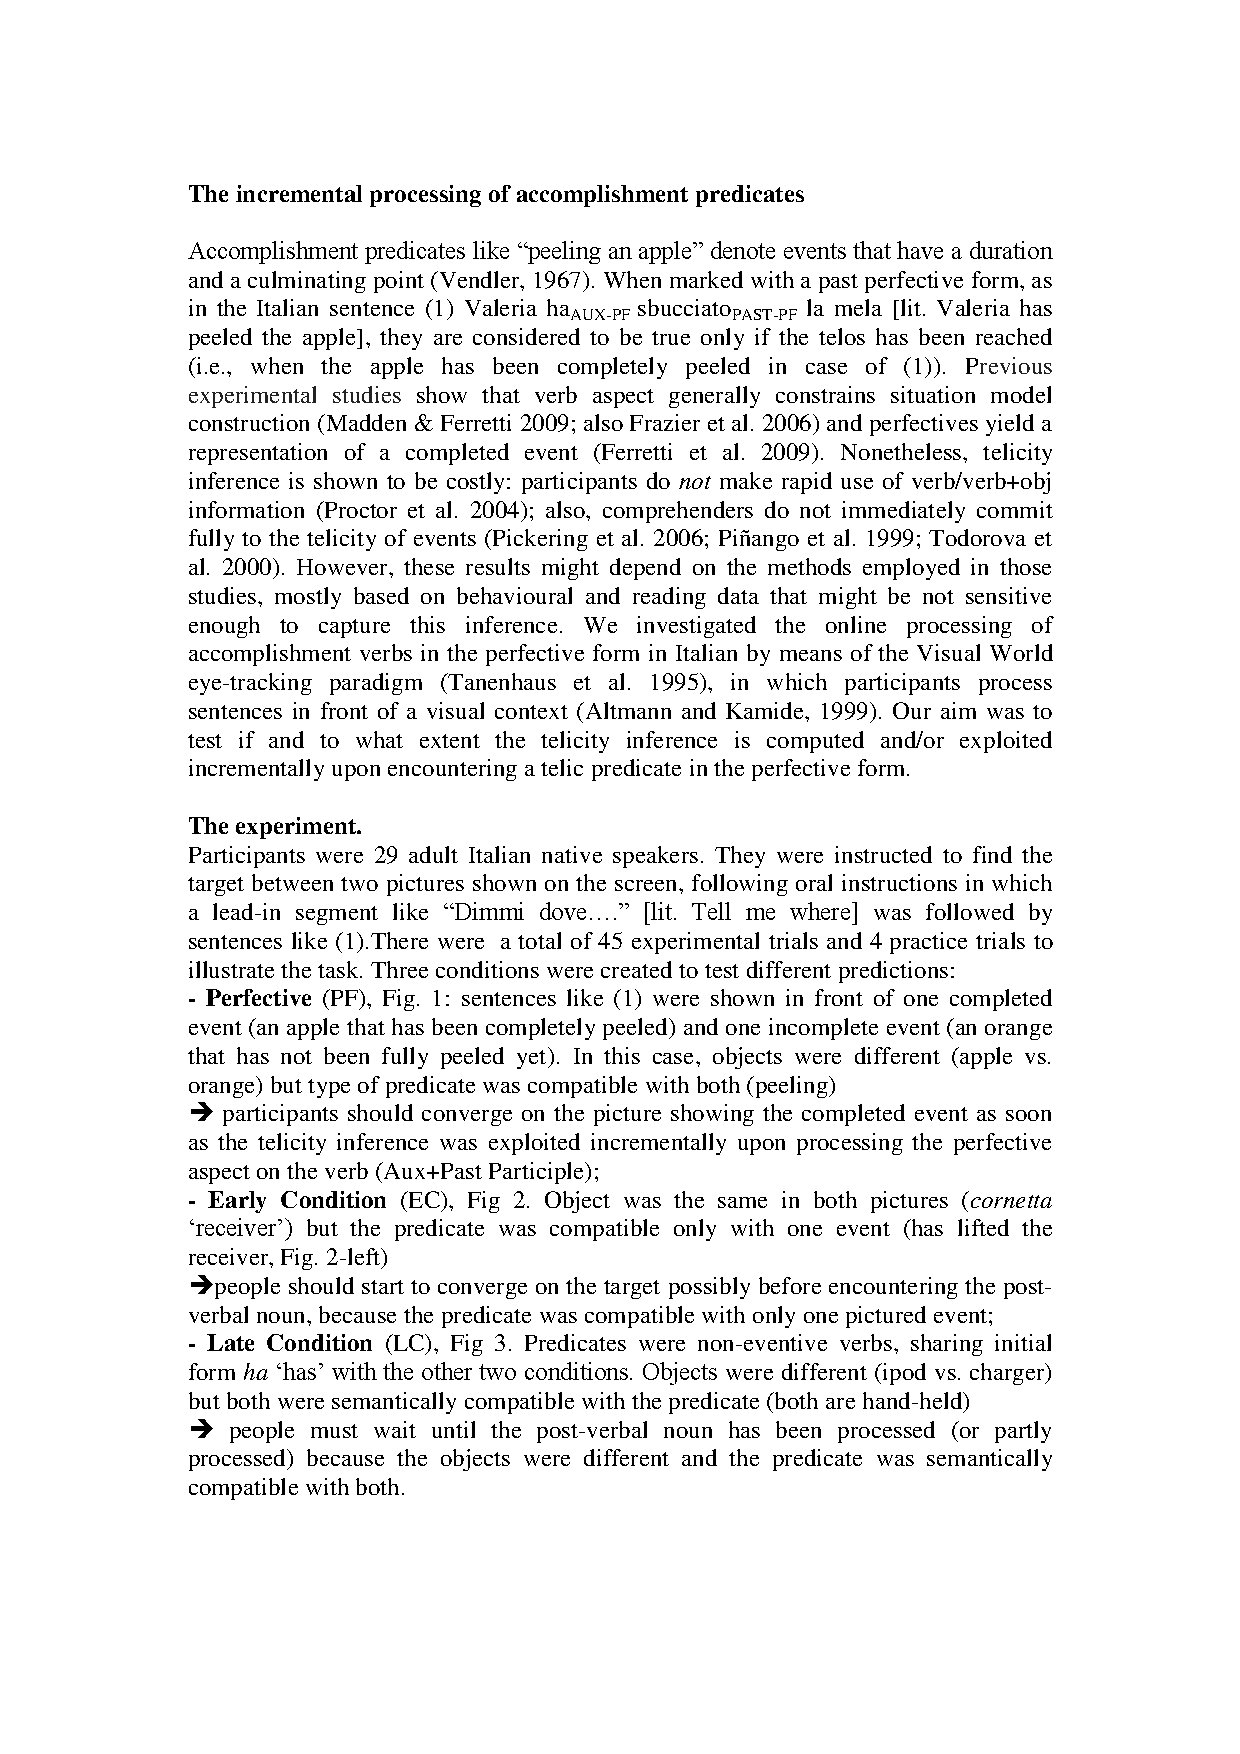
\includepdf[pagecommand={\thispagestyle{plain}}, pages=-]{03_ELC2016_paper_33.pdf}
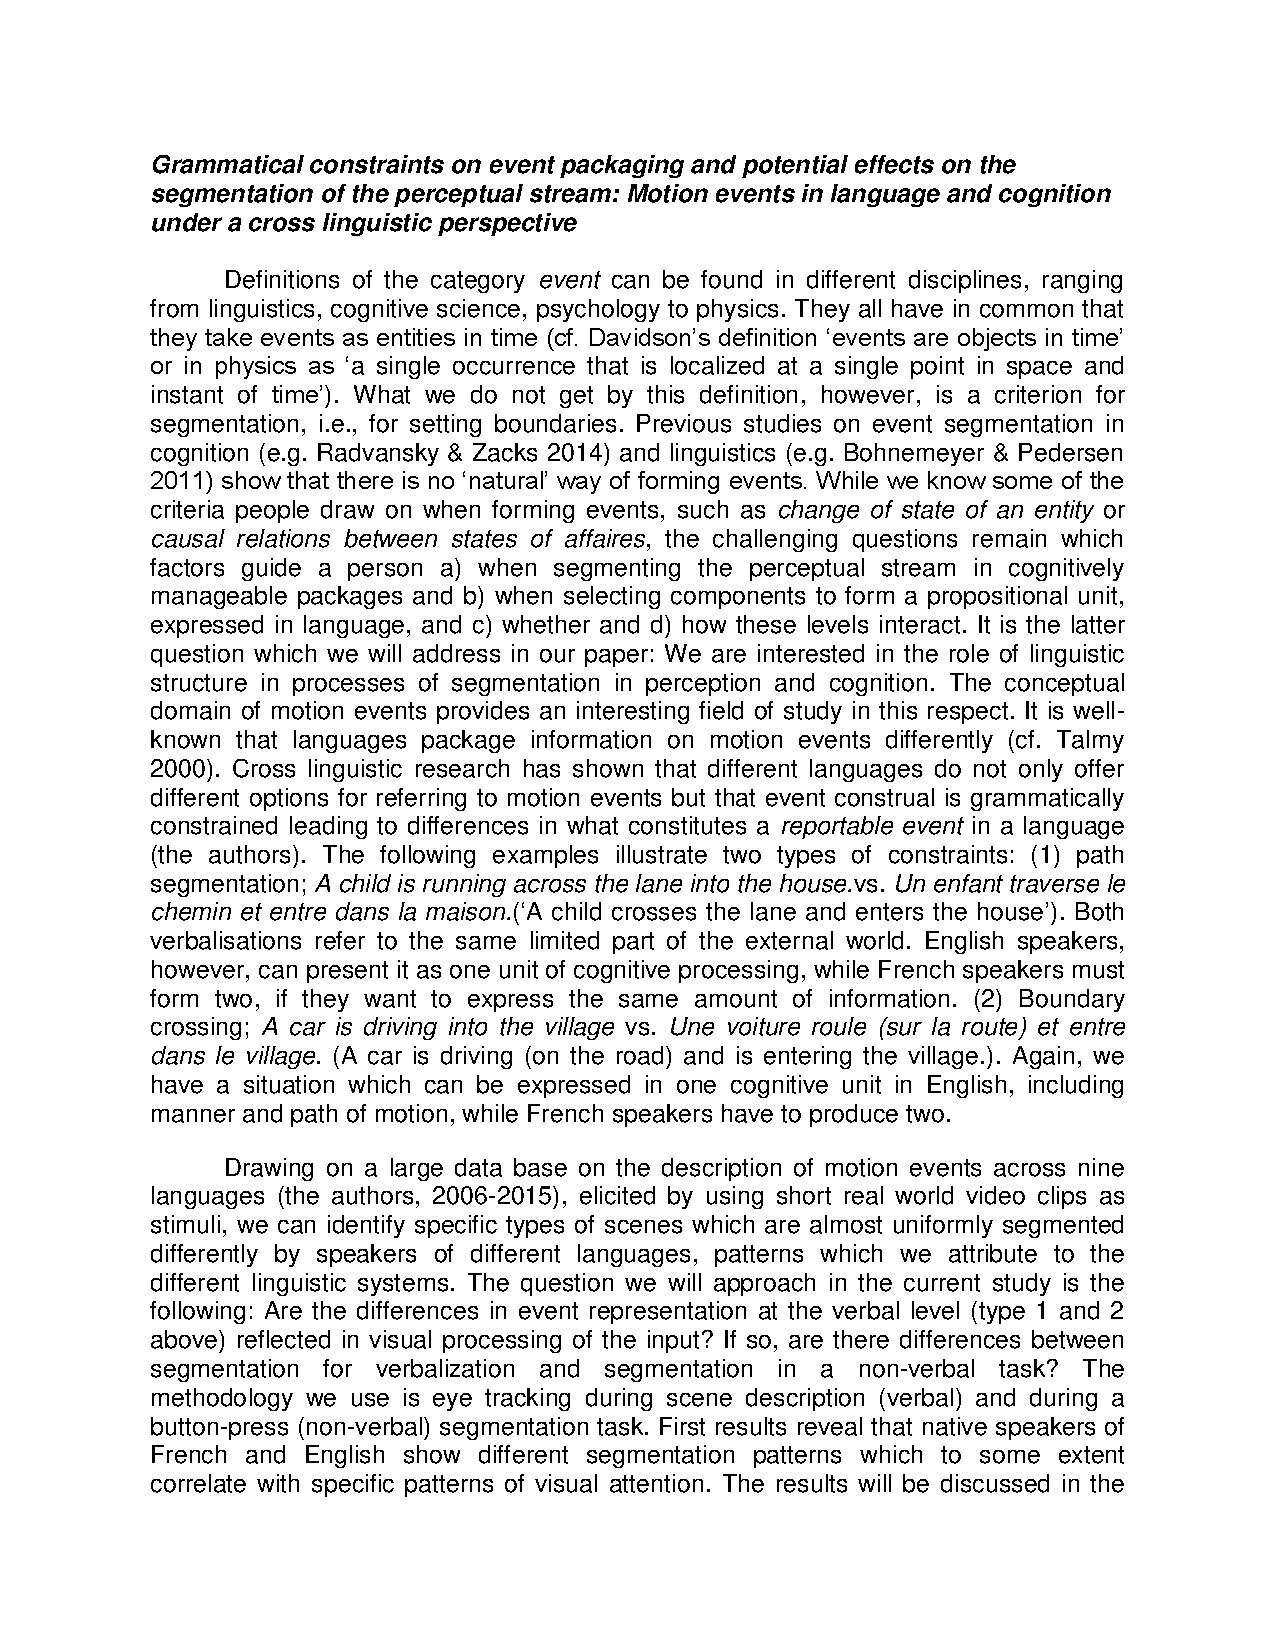
\includepdf[pagecommand={\thispagestyle{plain}}, pages=-]{04_ELC2016_paper_21.pdf}
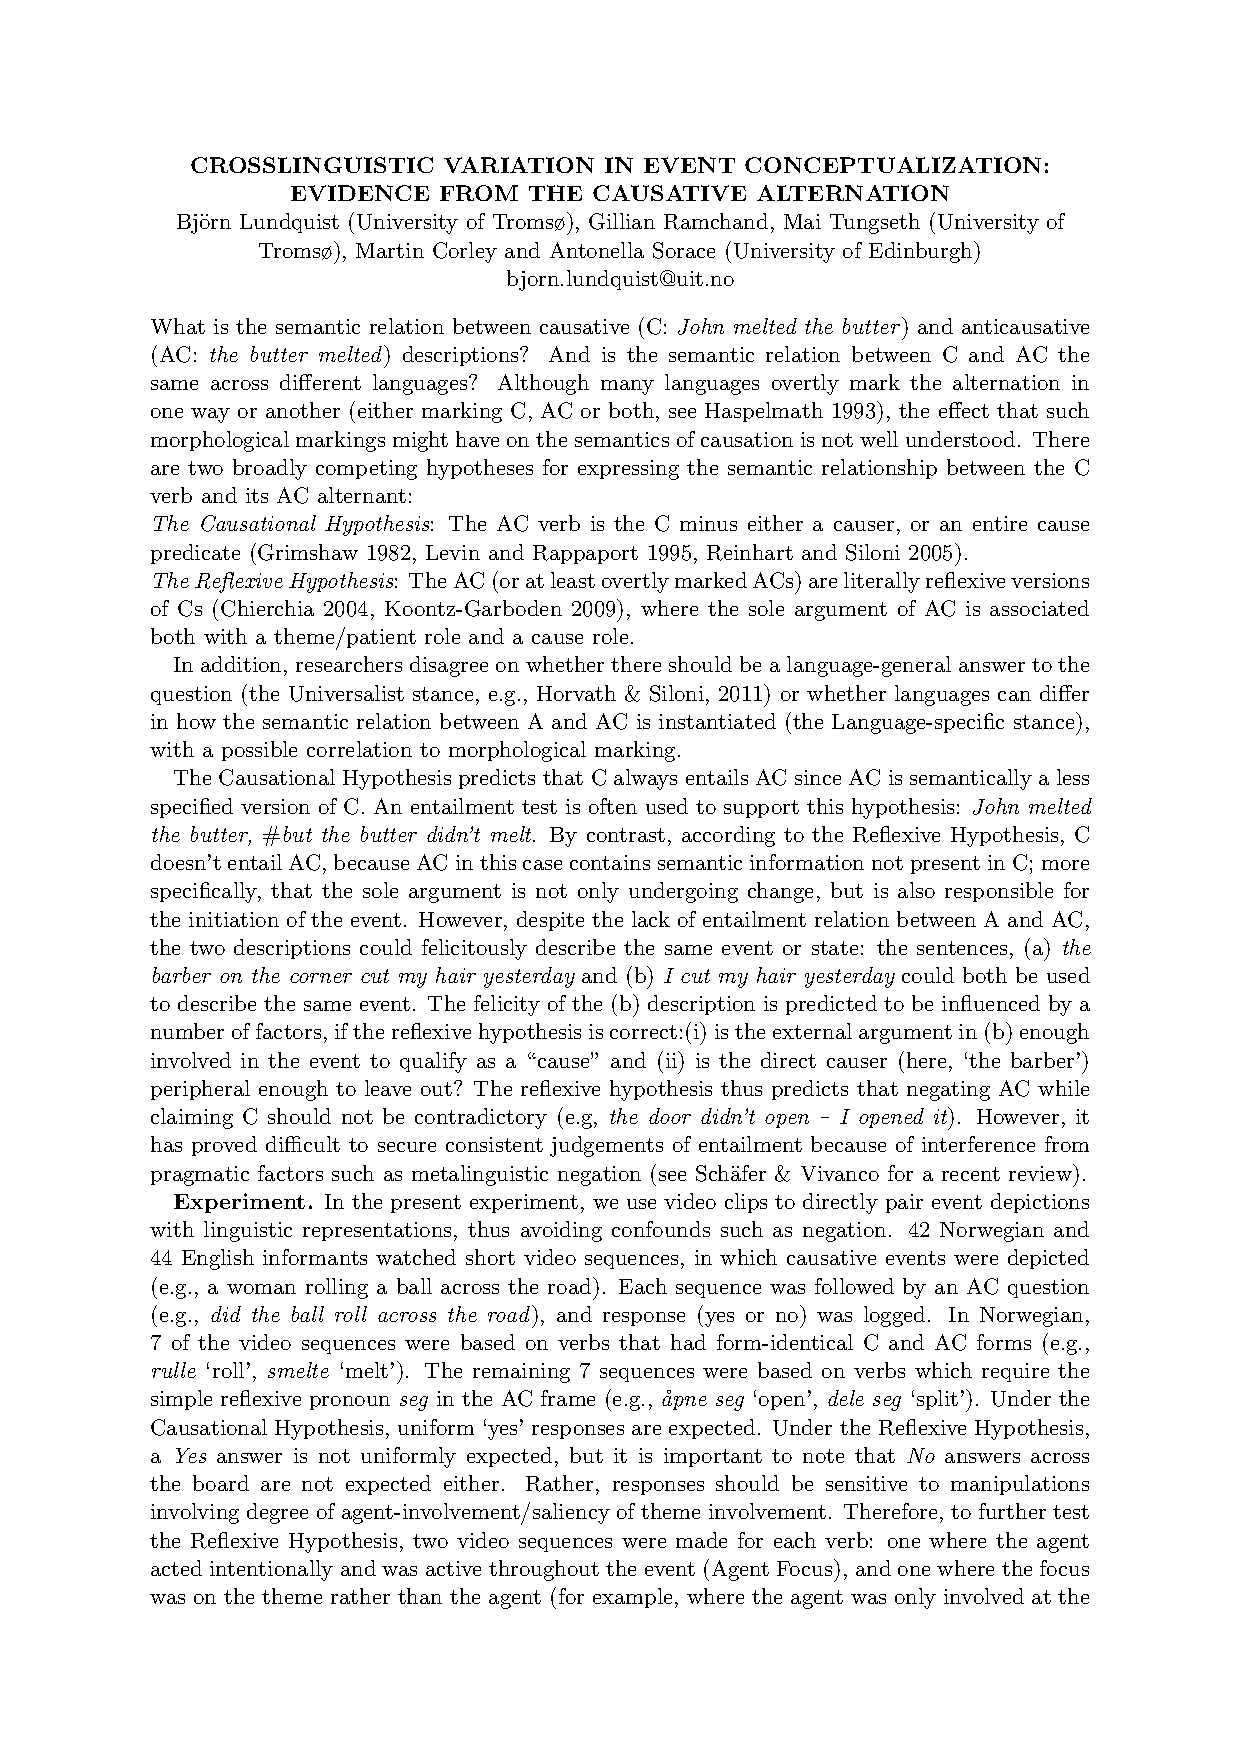
\includepdf[pagecommand={\thispagestyle{plain}}, pages=-]{05_videoabstract3.pdf}
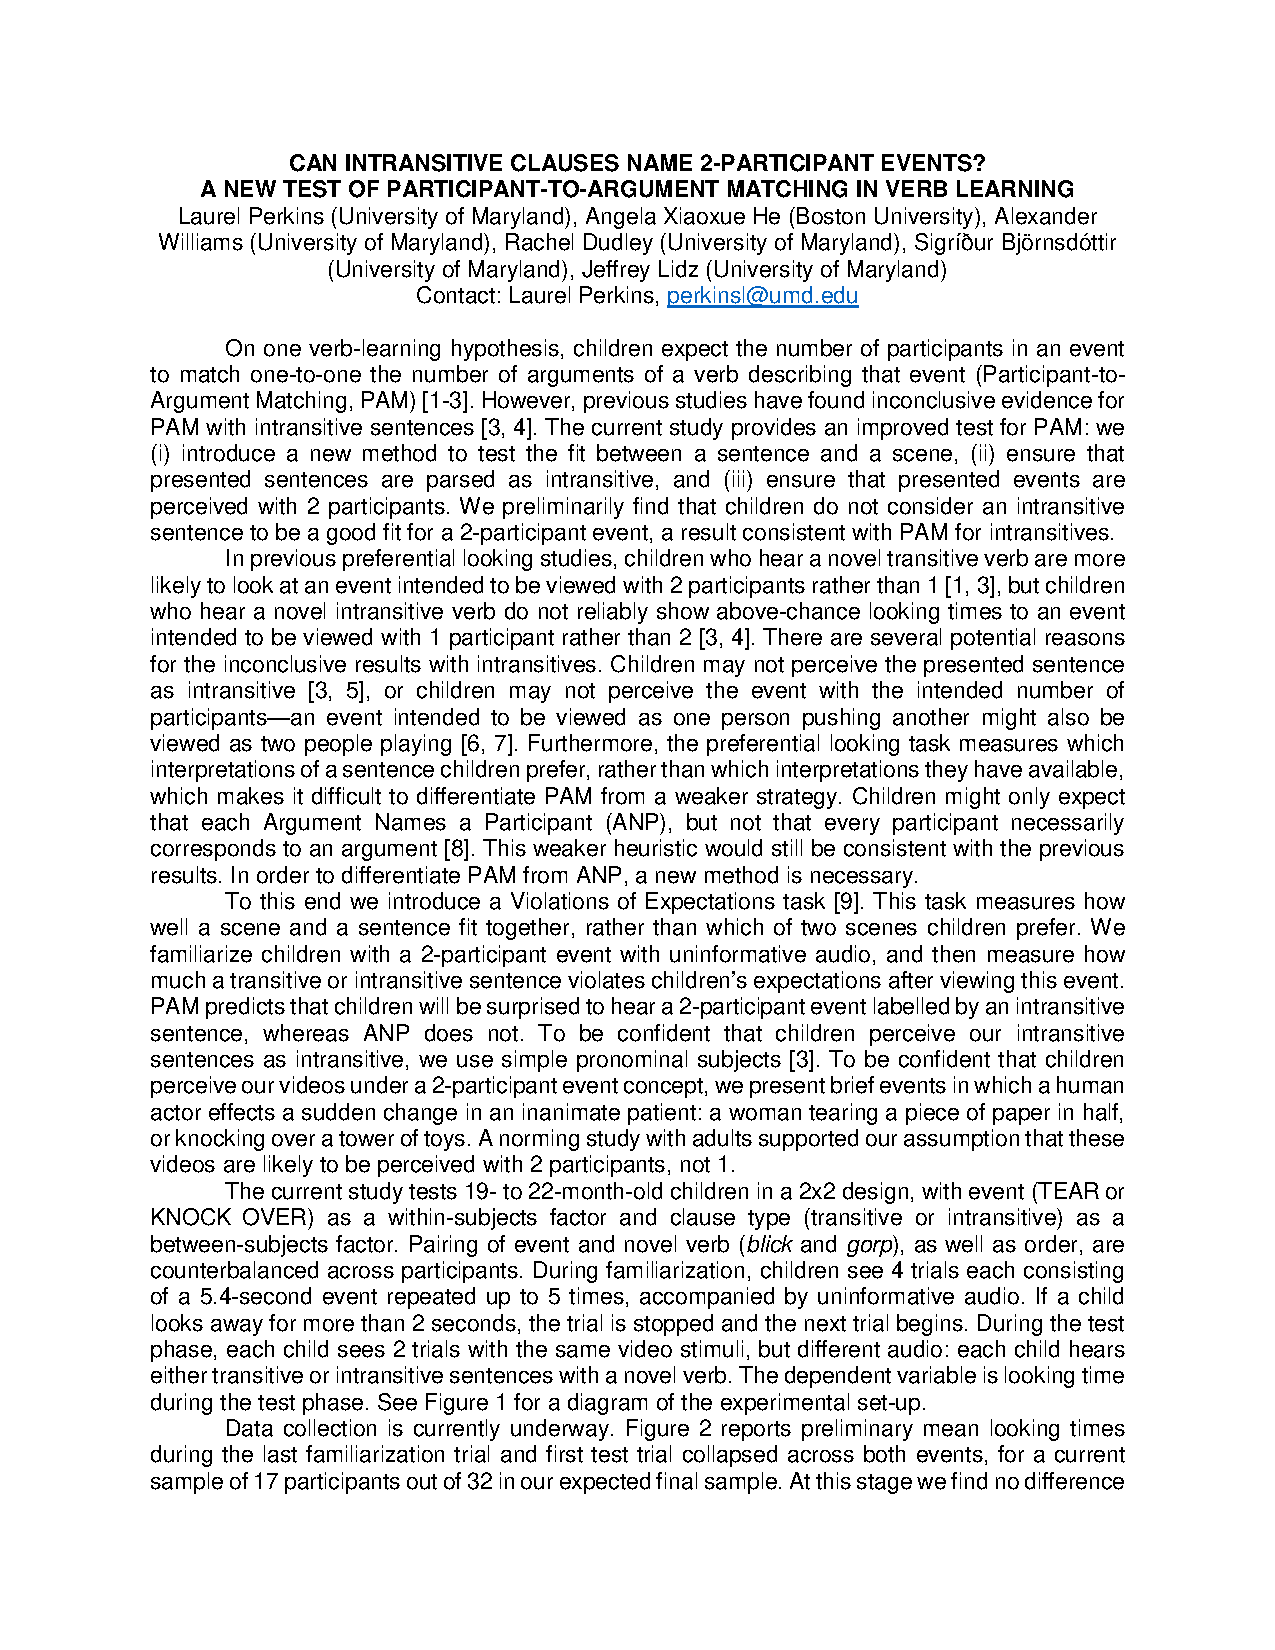
\includepdf[pagecommand={\thispagestyle{plain}}, pages=-]{06_ELC2016-PerkinsEtAl-Abstract-FINAL.pdf}
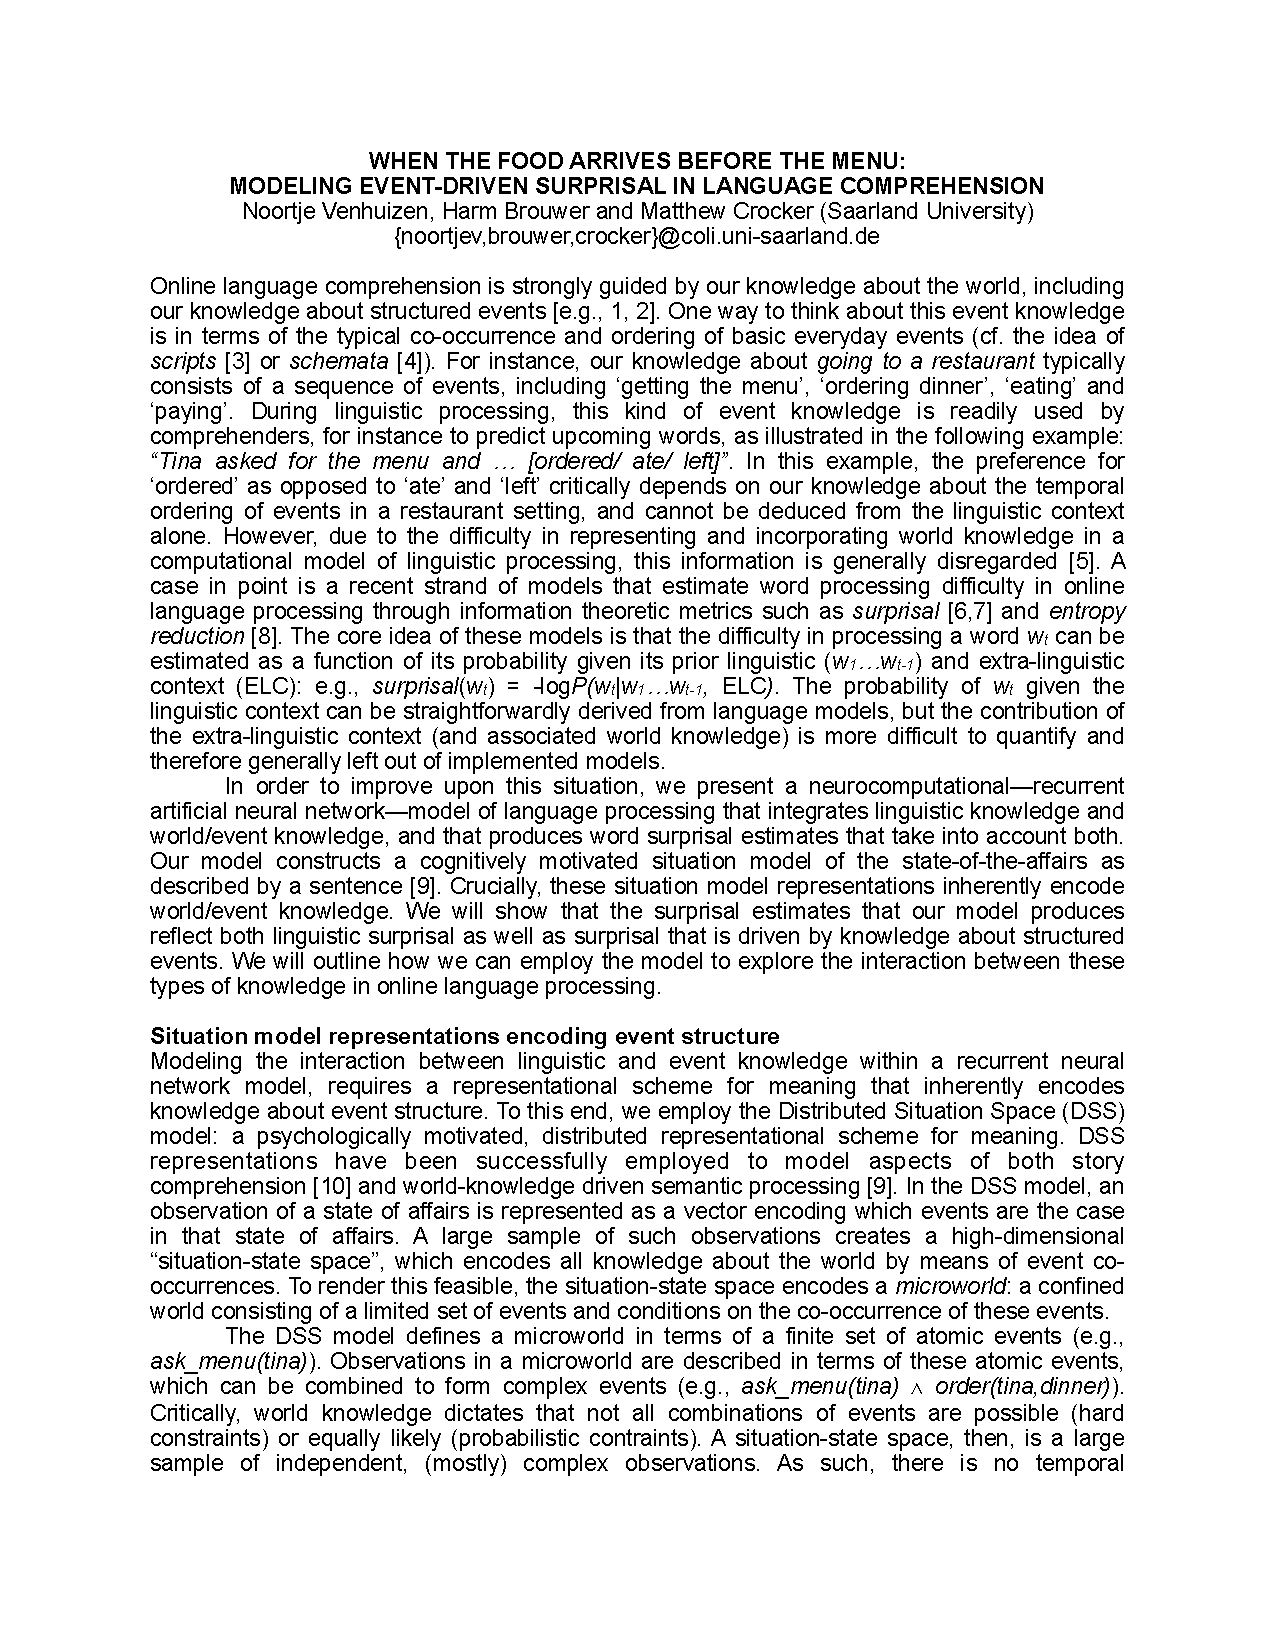
\includepdf[pagecommand={\thispagestyle{plain}}, pages=-]{07_abstract_ELC2016_final.pdf}
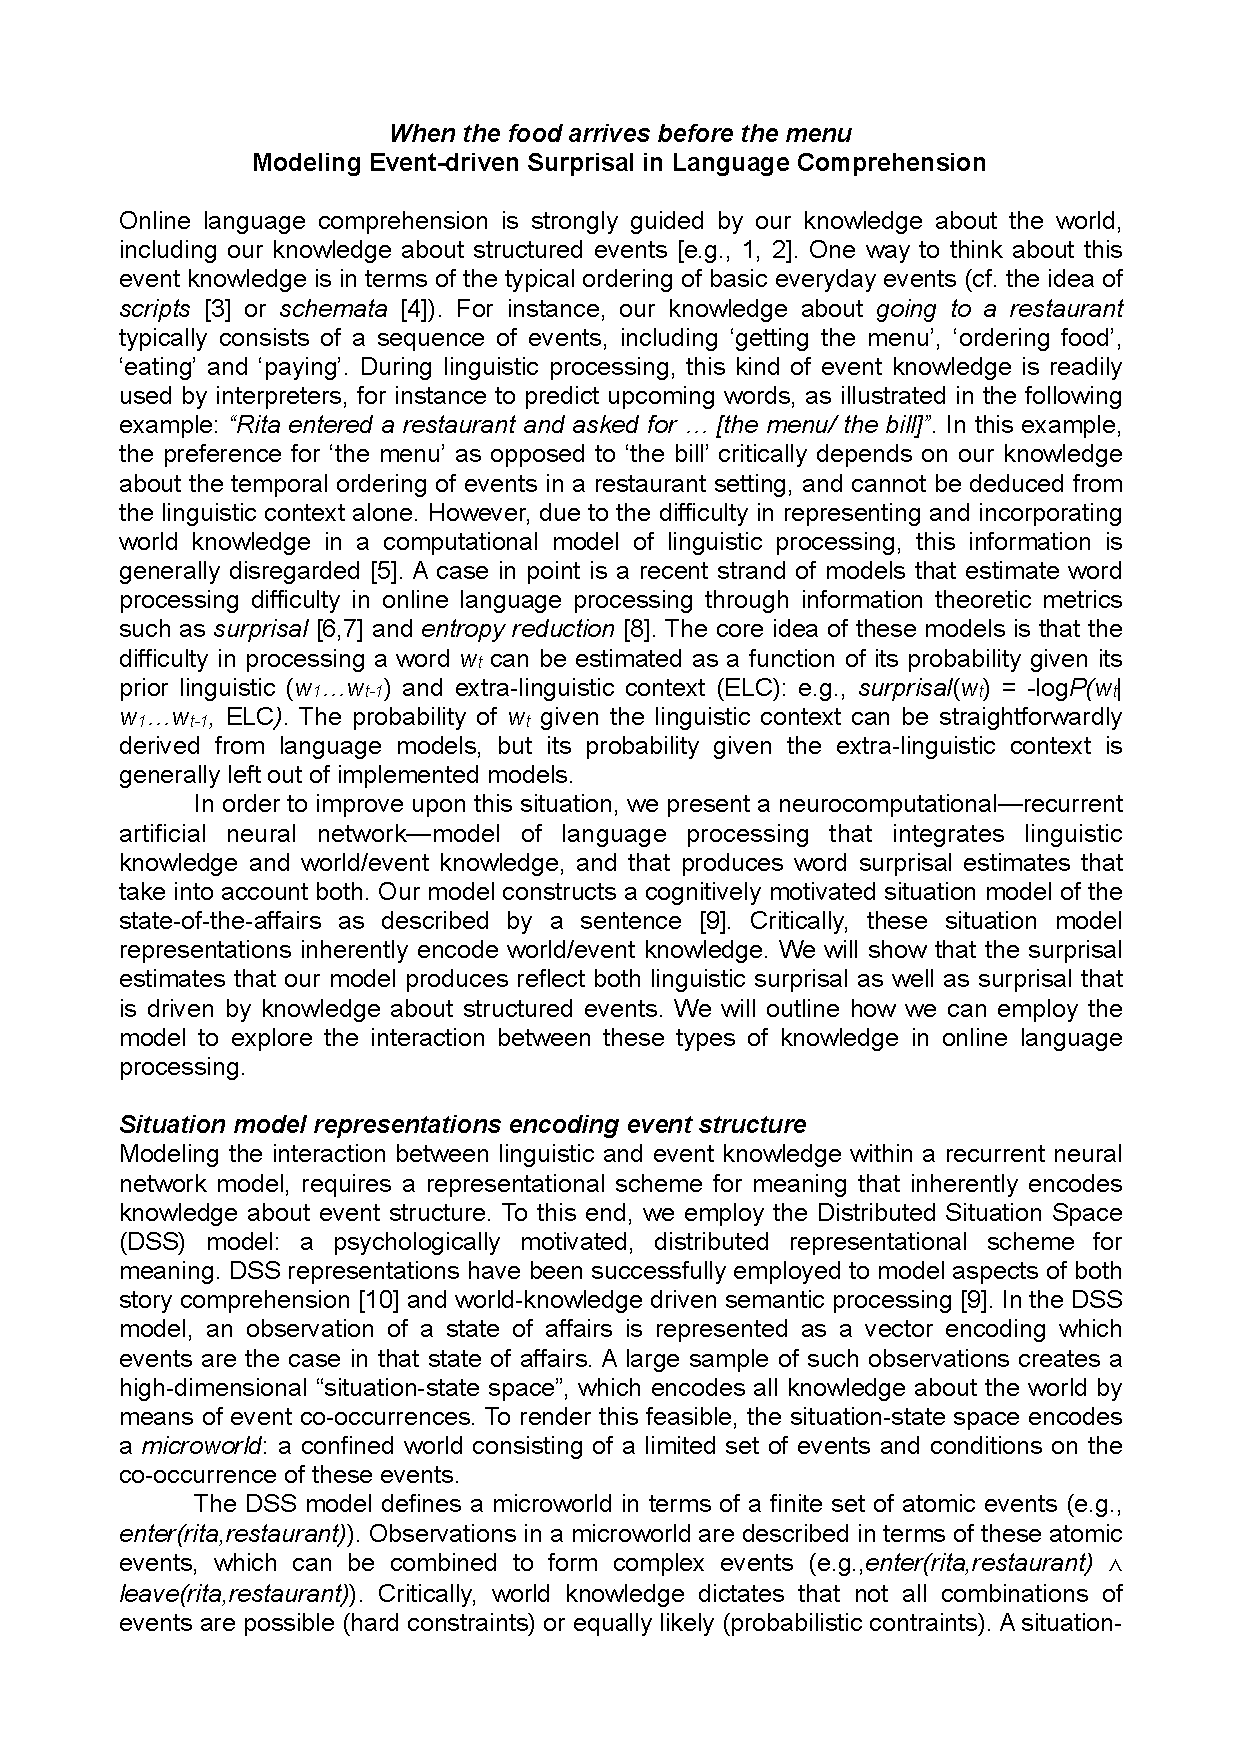
\includepdf[pagecommand={\thispagestyle{plain}}, pages=-]{07_ELC2016_paper_18.pdf}
\includepdf[pagecommand={\thispagestyle{plain}}, pages=-]{"08_UTP_ELC2016 - final".pdf}
\includepdf[pagecommand={\thispagestyle{plain}}, pages=-]{"09_Event parsing and verb learning".pdf}
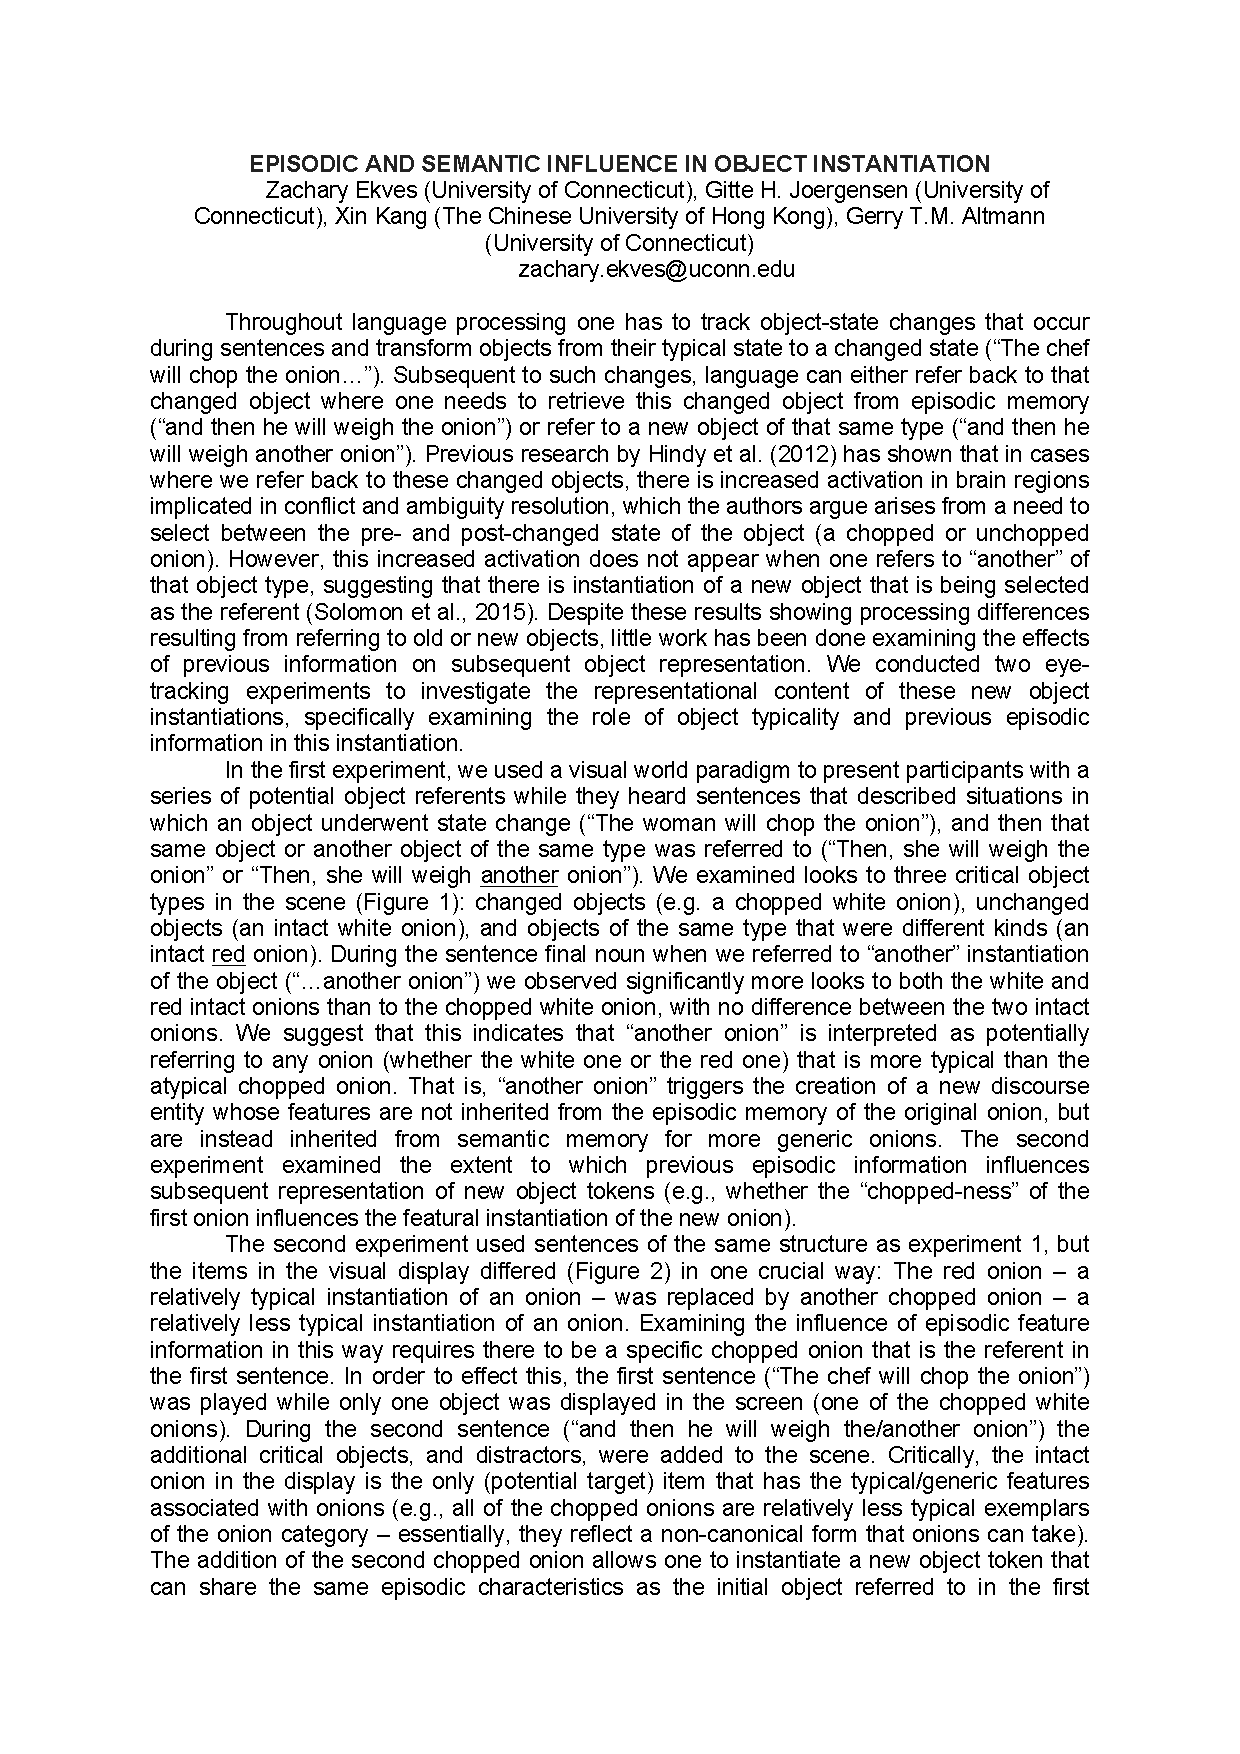
\includepdf[pagecommand={\thispagestyle{plain}}, pages=-]{10_FinalELCAbstract.pdf}
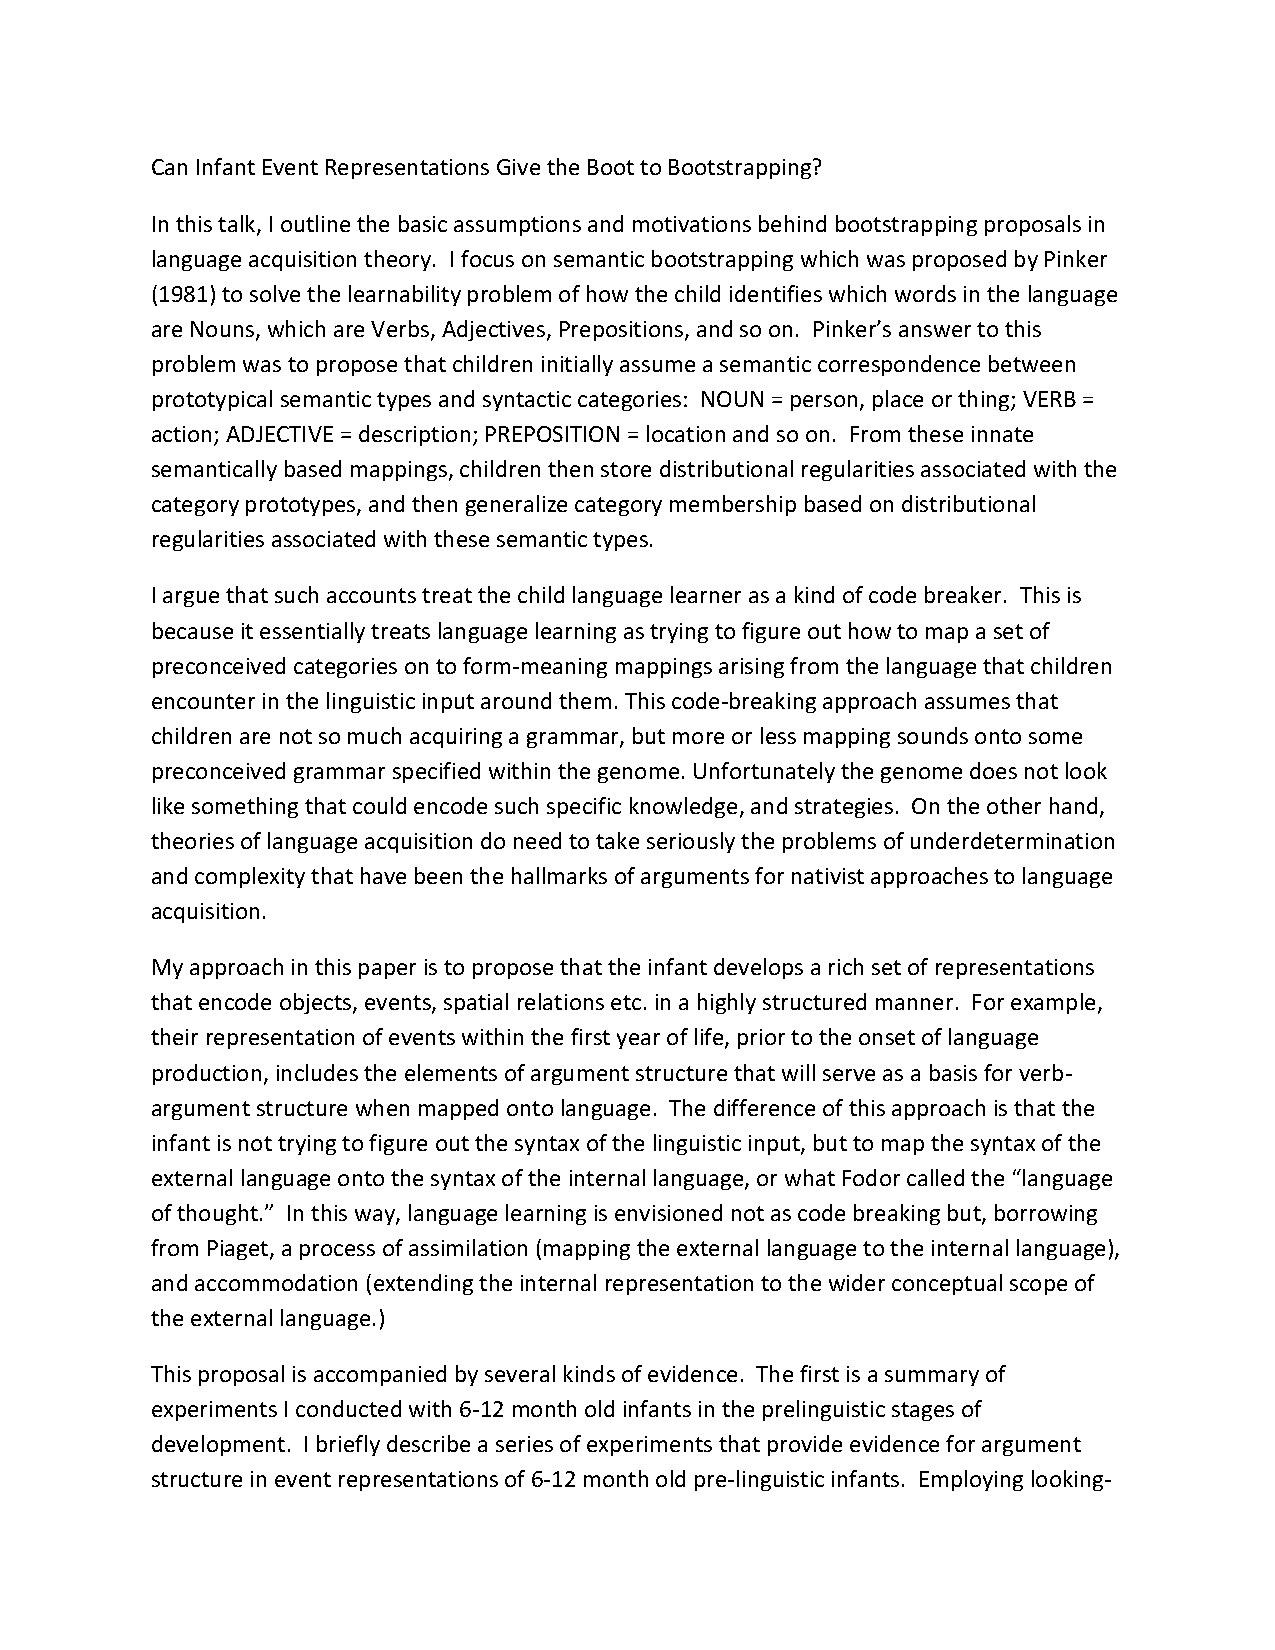
\includepdf[pagecommand={\thispagestyle{plain}}, pages=-]{12_ELC2016_paper_53.pdf}
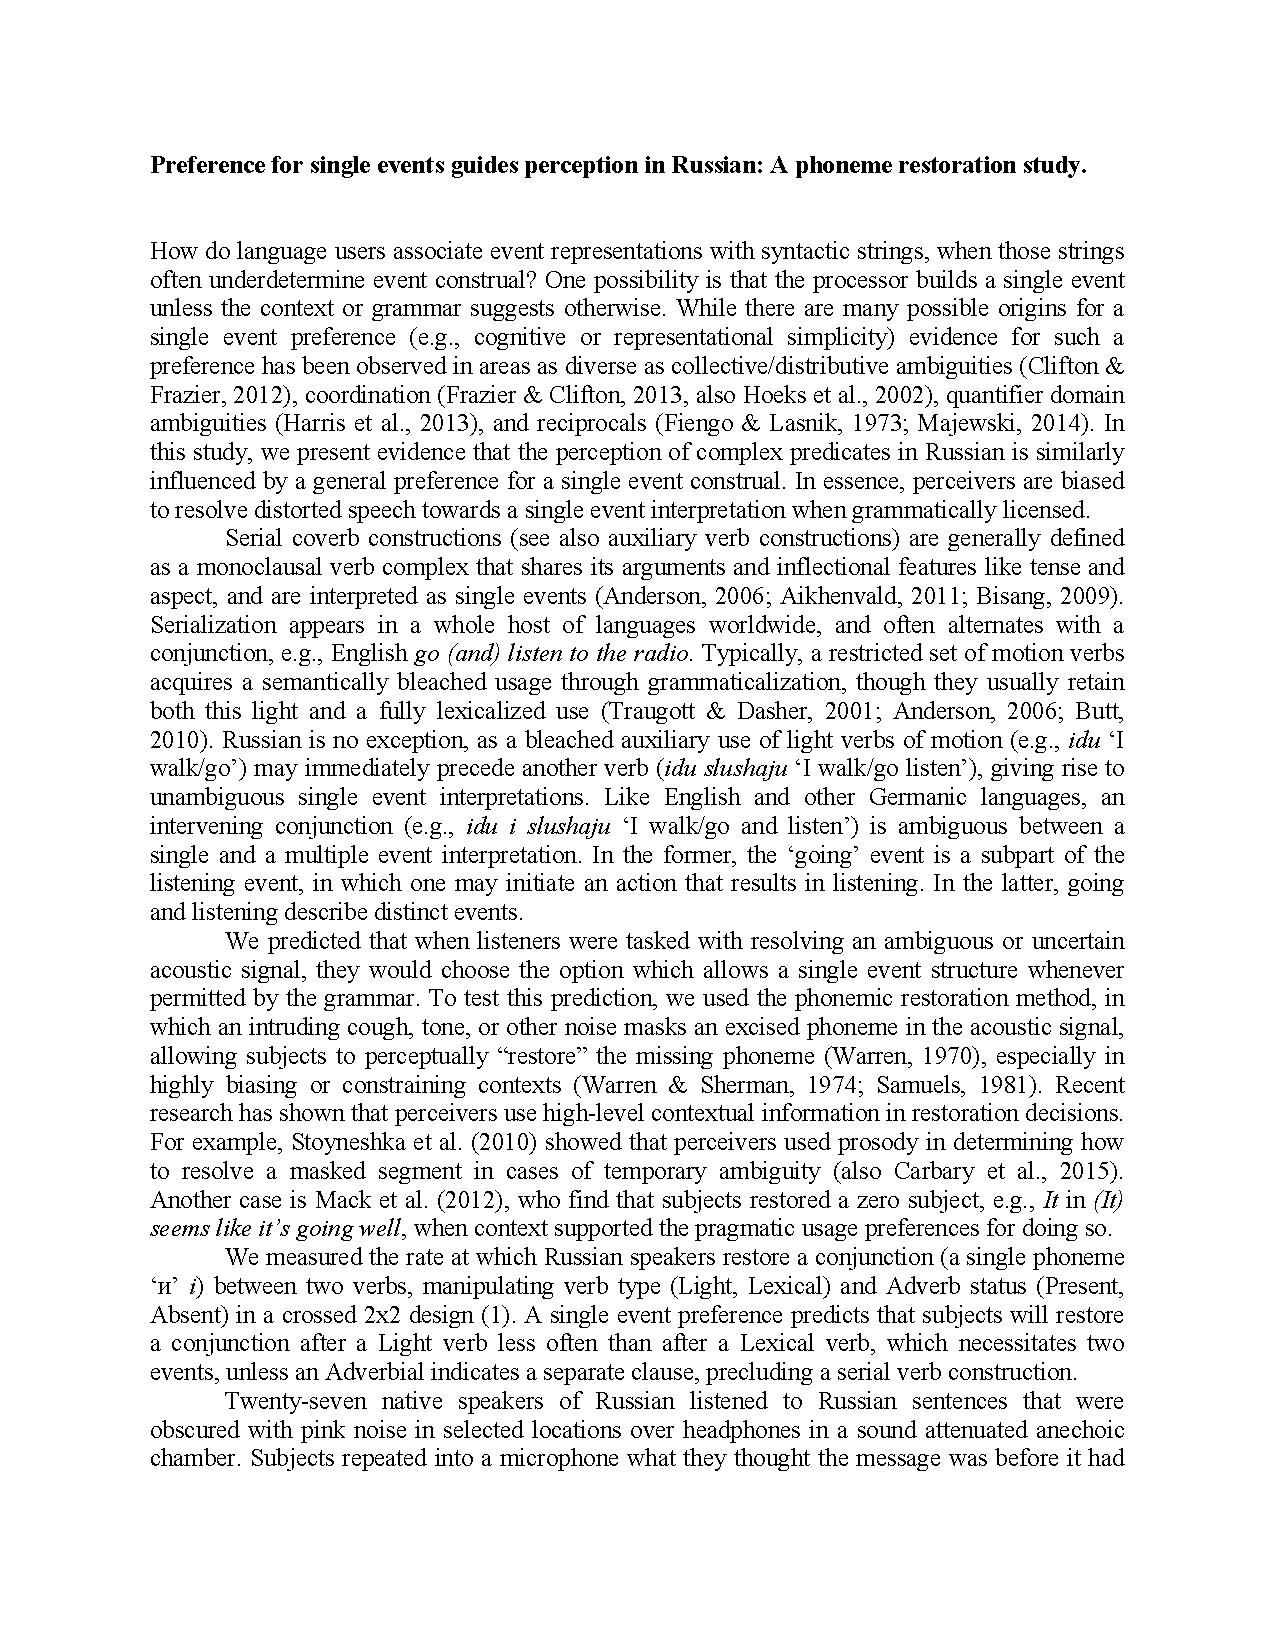
\includepdf[pagecommand={\thispagestyle{plain}}, pages=-]{13_ELC2016_paper_13.pdf}
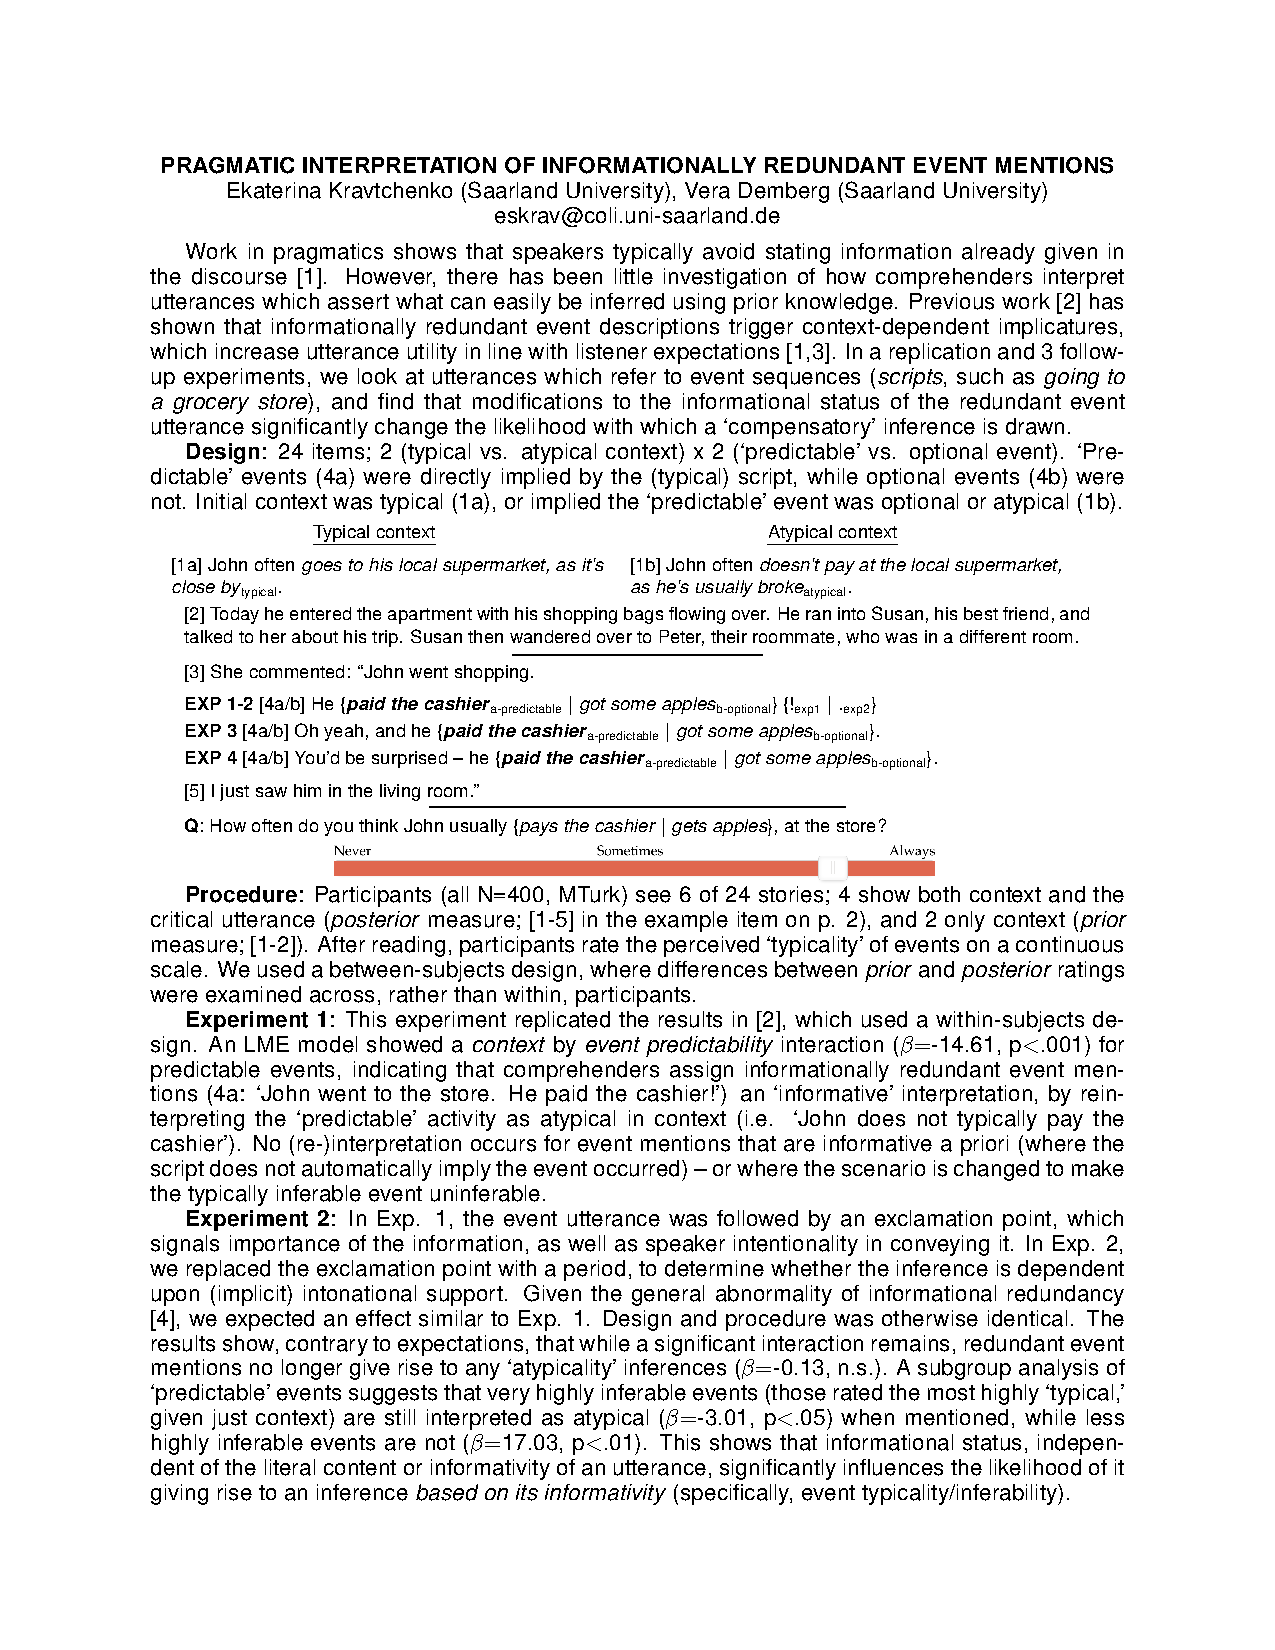
\includepdf[pagecommand={\thispagestyle{plain}}, pages=-]{14_Kravtchenko_Demberg_CUNY_2016_final_abstract.pdf}
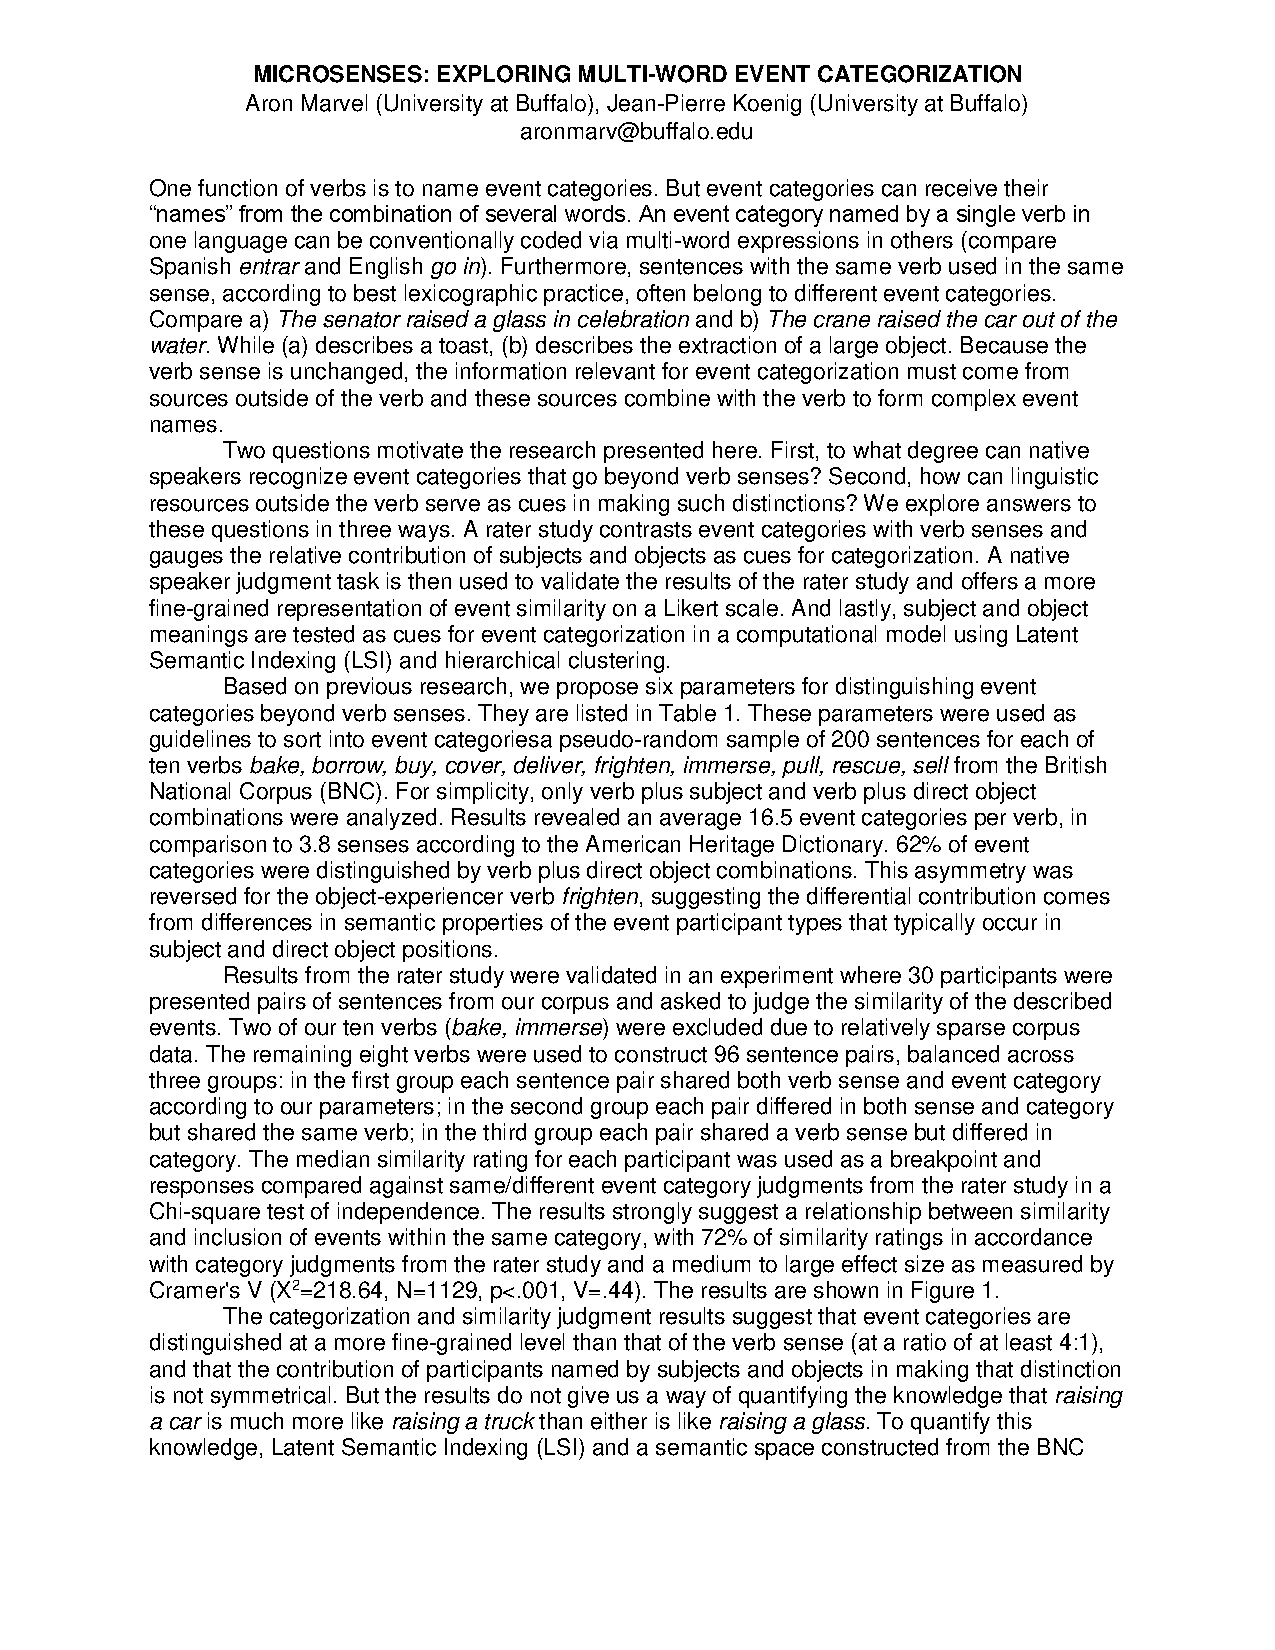
\includepdf[pagecommand={\thispagestyle{plain}}, pages=-]{15_Marvel_Koenig_ELC_2016_abstract.pdf}
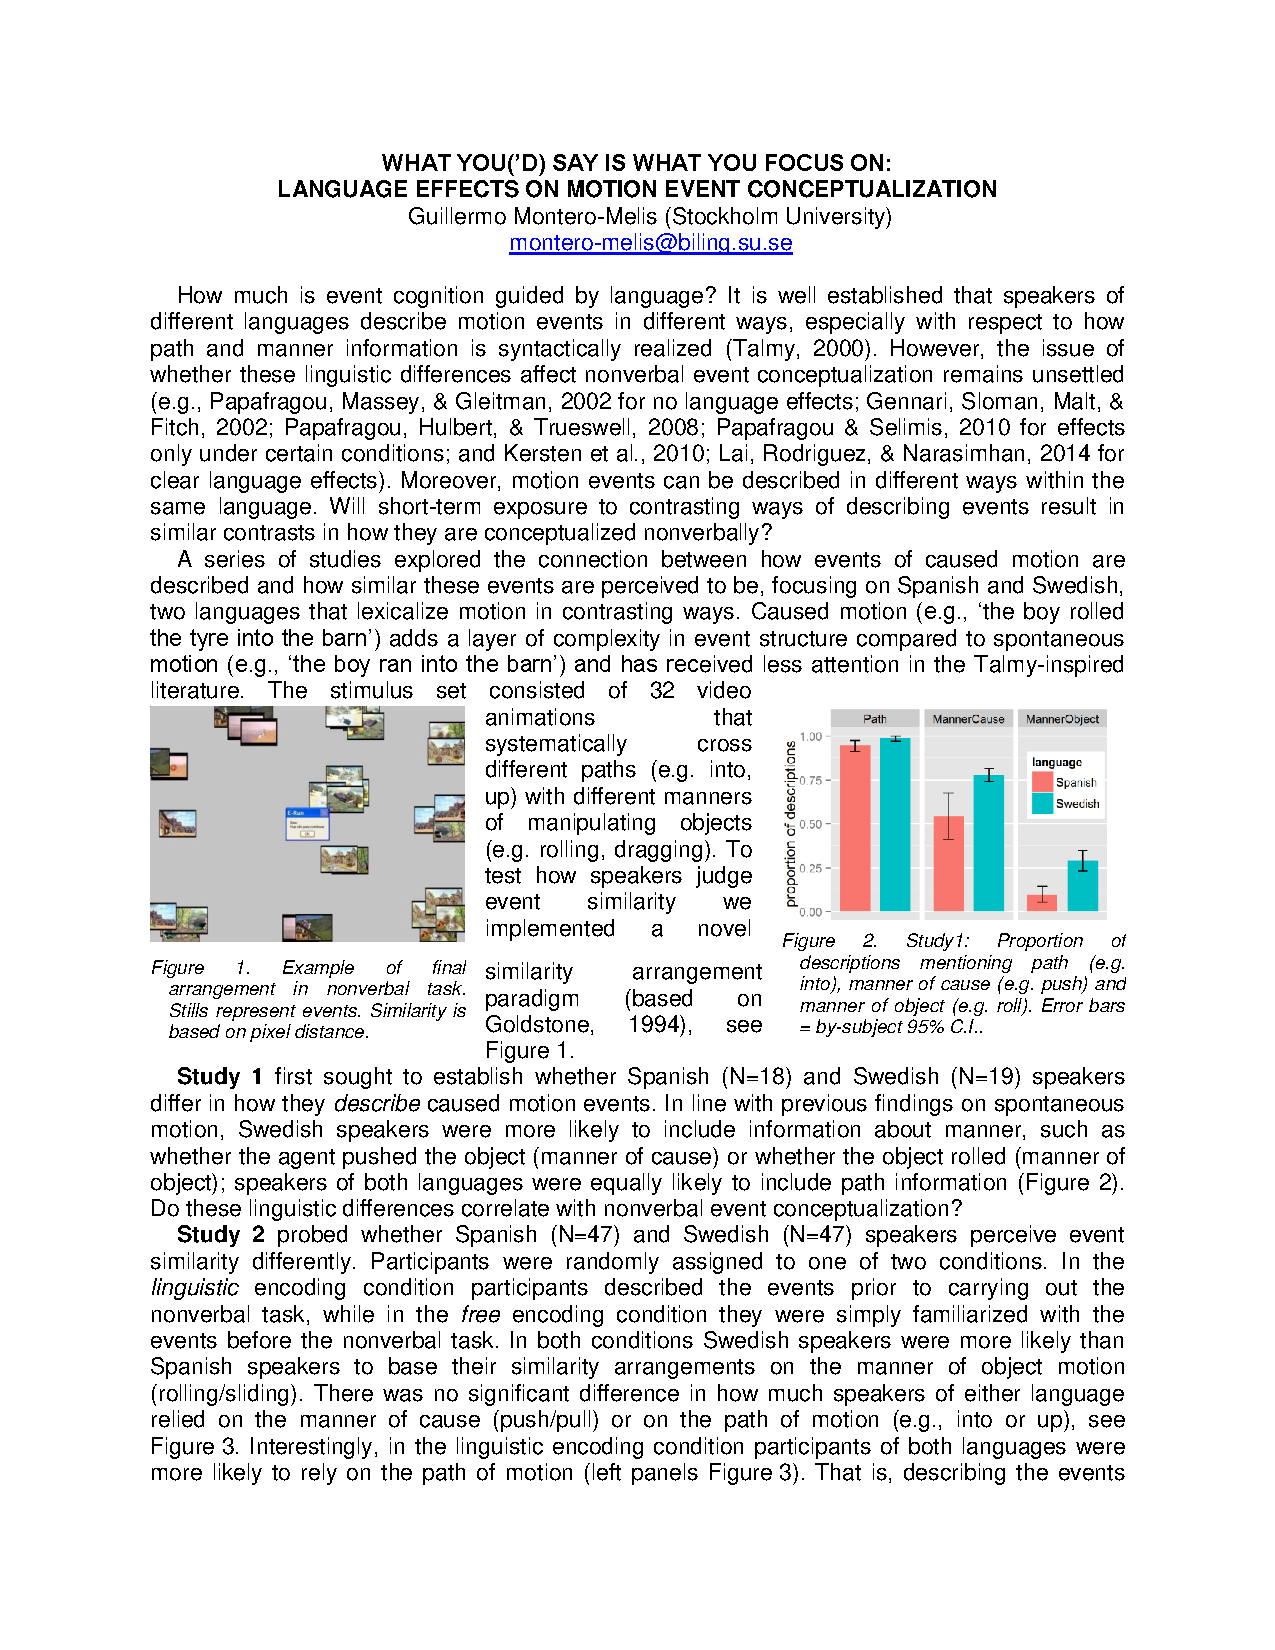
\includepdf[pagecommand={\thispagestyle{plain}}, pages=-]{16_montero-melis_what-you-say_final_160205.pdf}
\includepdf[pagecommand={\thispagestyle{plain}}, pages=-]{"17_Potapova Boroditsky Events in Language and Cognition Formatted".pdf}
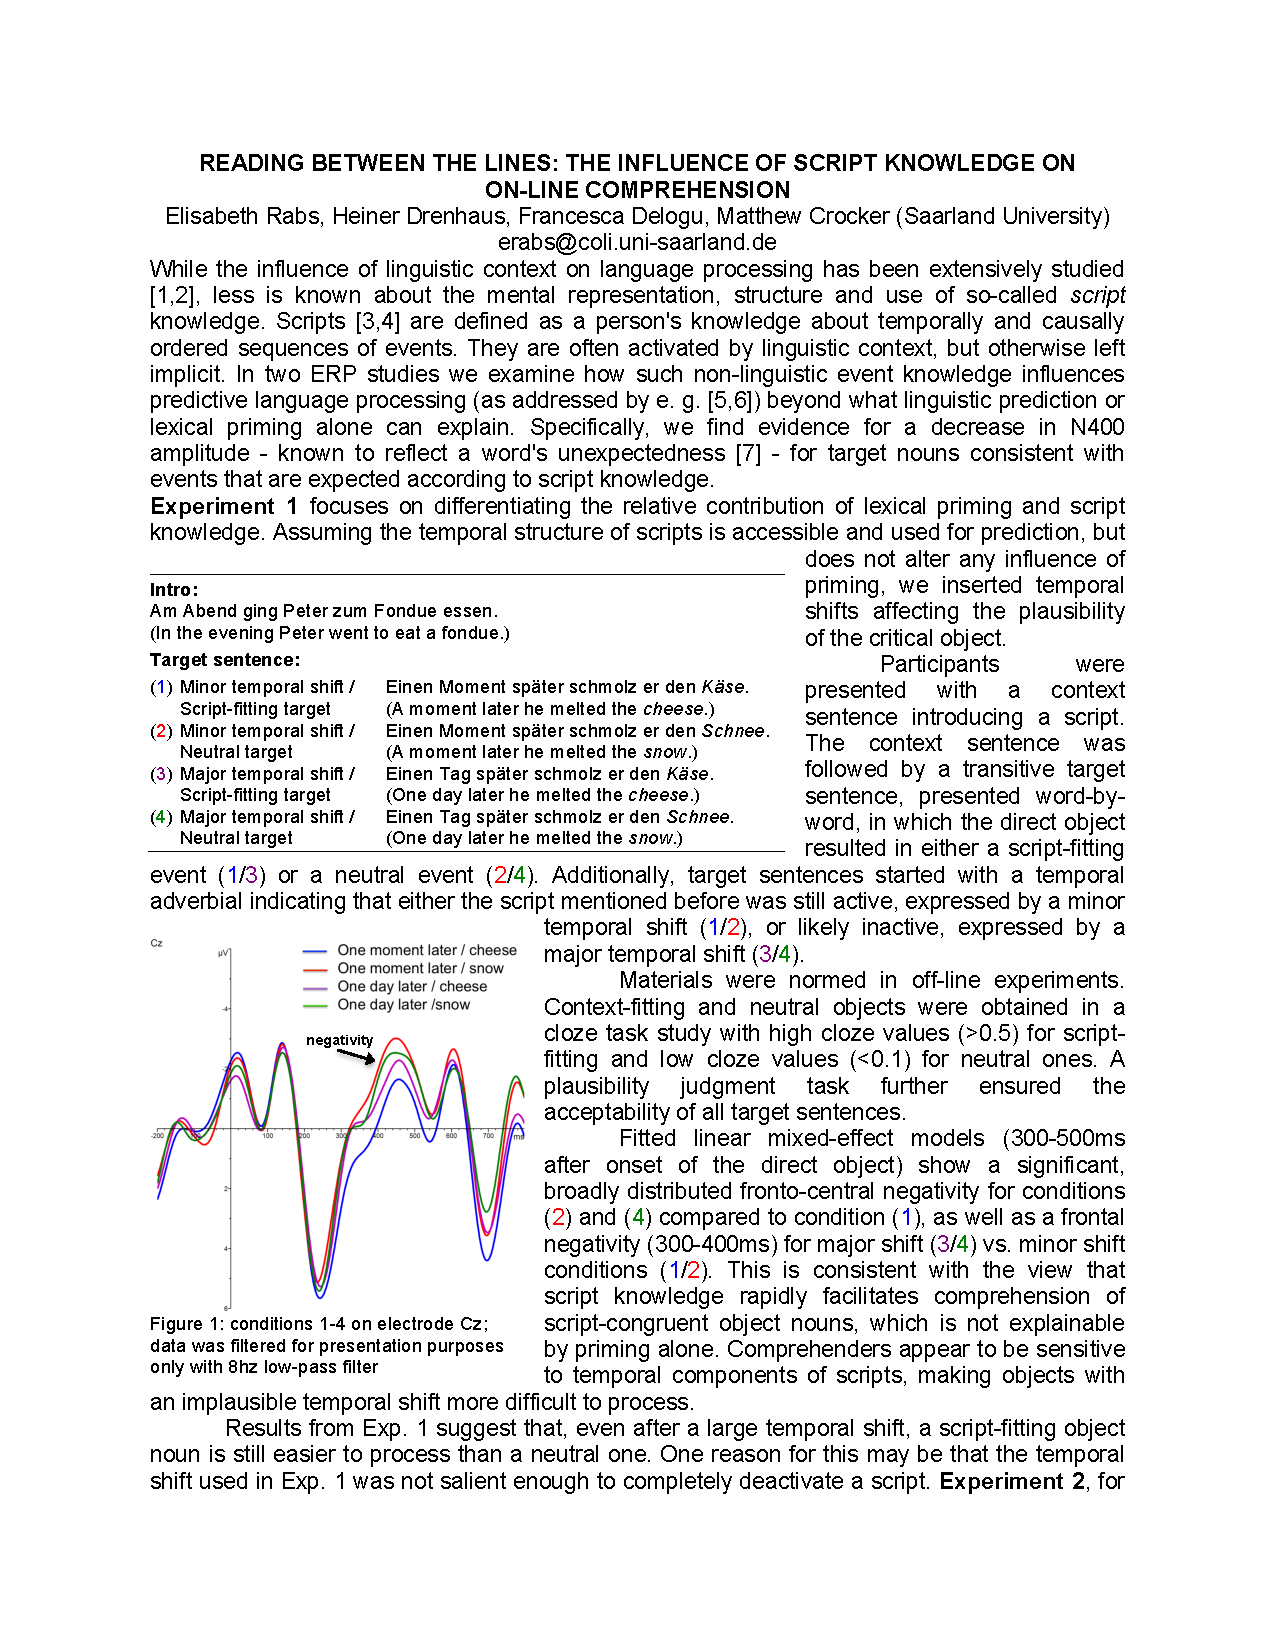
\includepdf[pagecommand={\thispagestyle{plain}}, pages=-]{18_ELC2016_ER_revised.pdf}
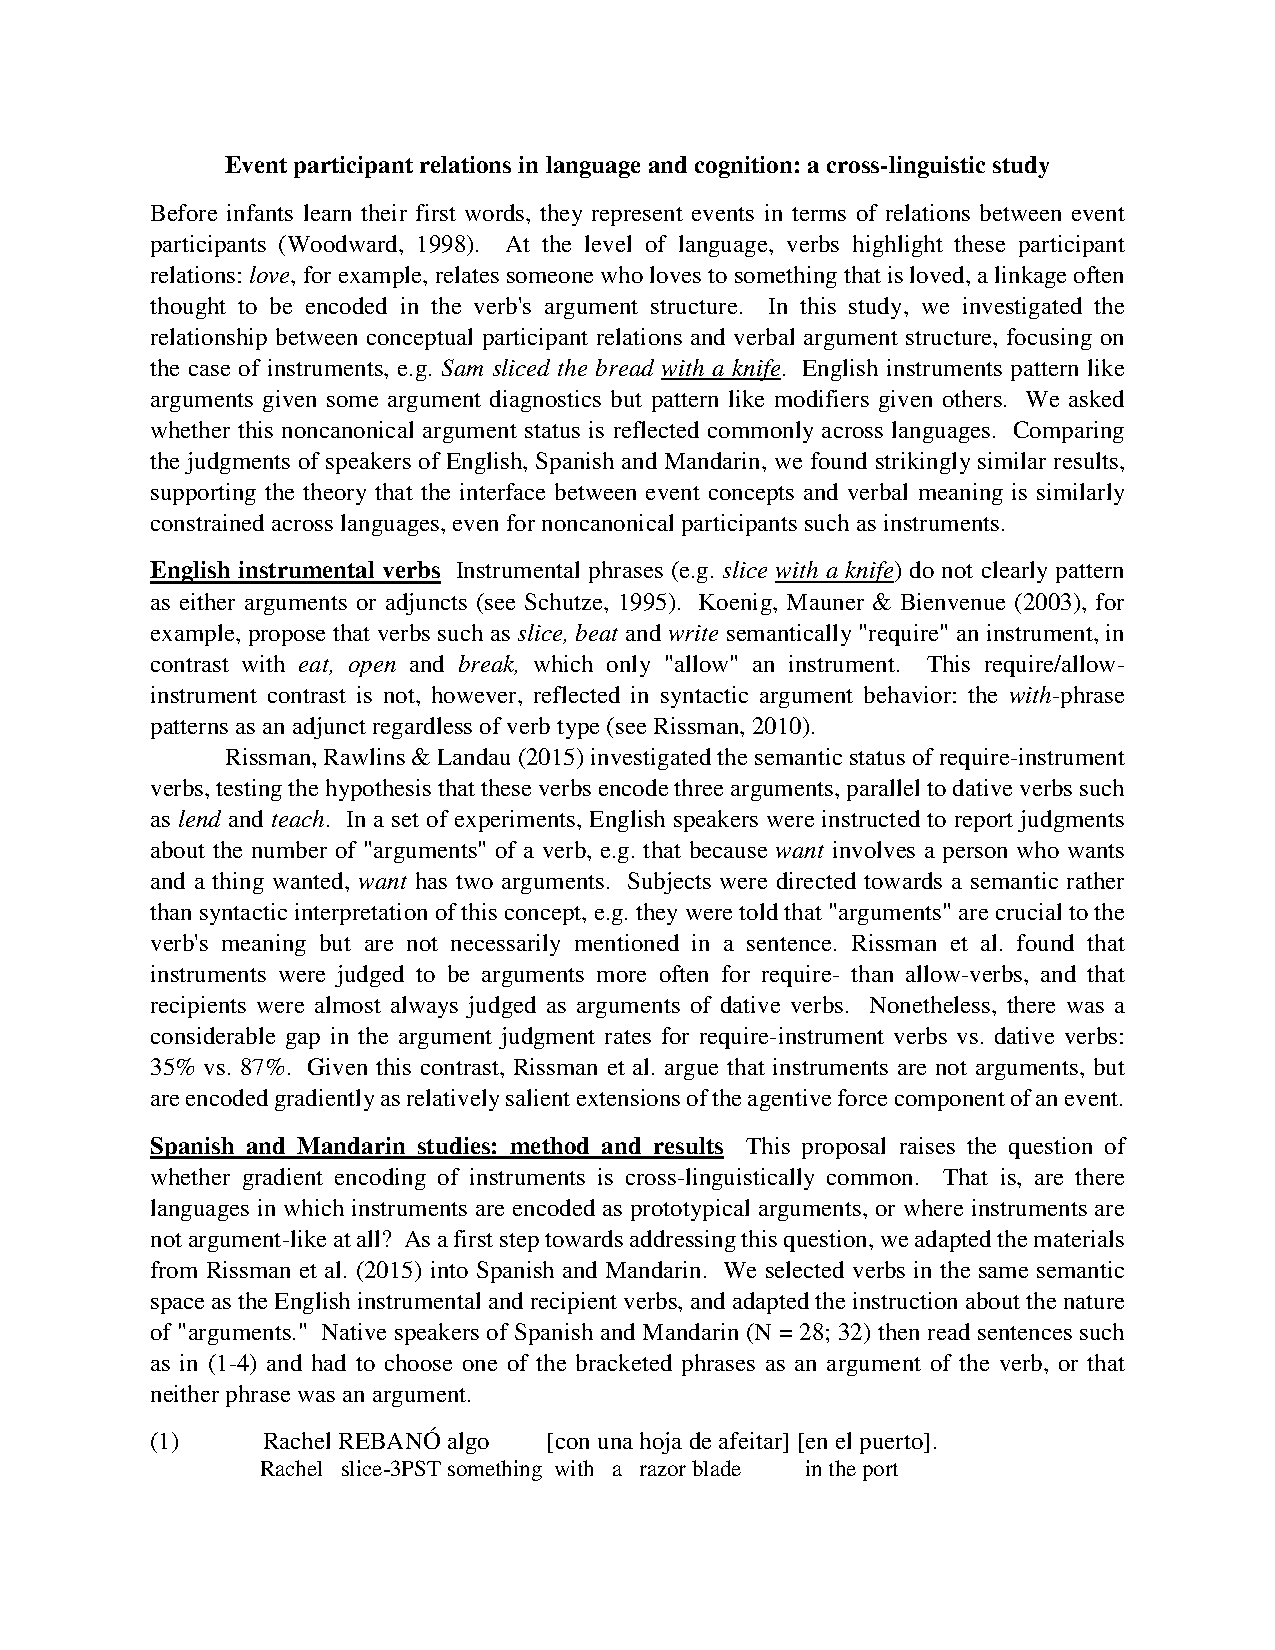
\includepdf[pagecommand={\thispagestyle{plain}}, pages=-]{19_ELC2016_paper_37.pdf}
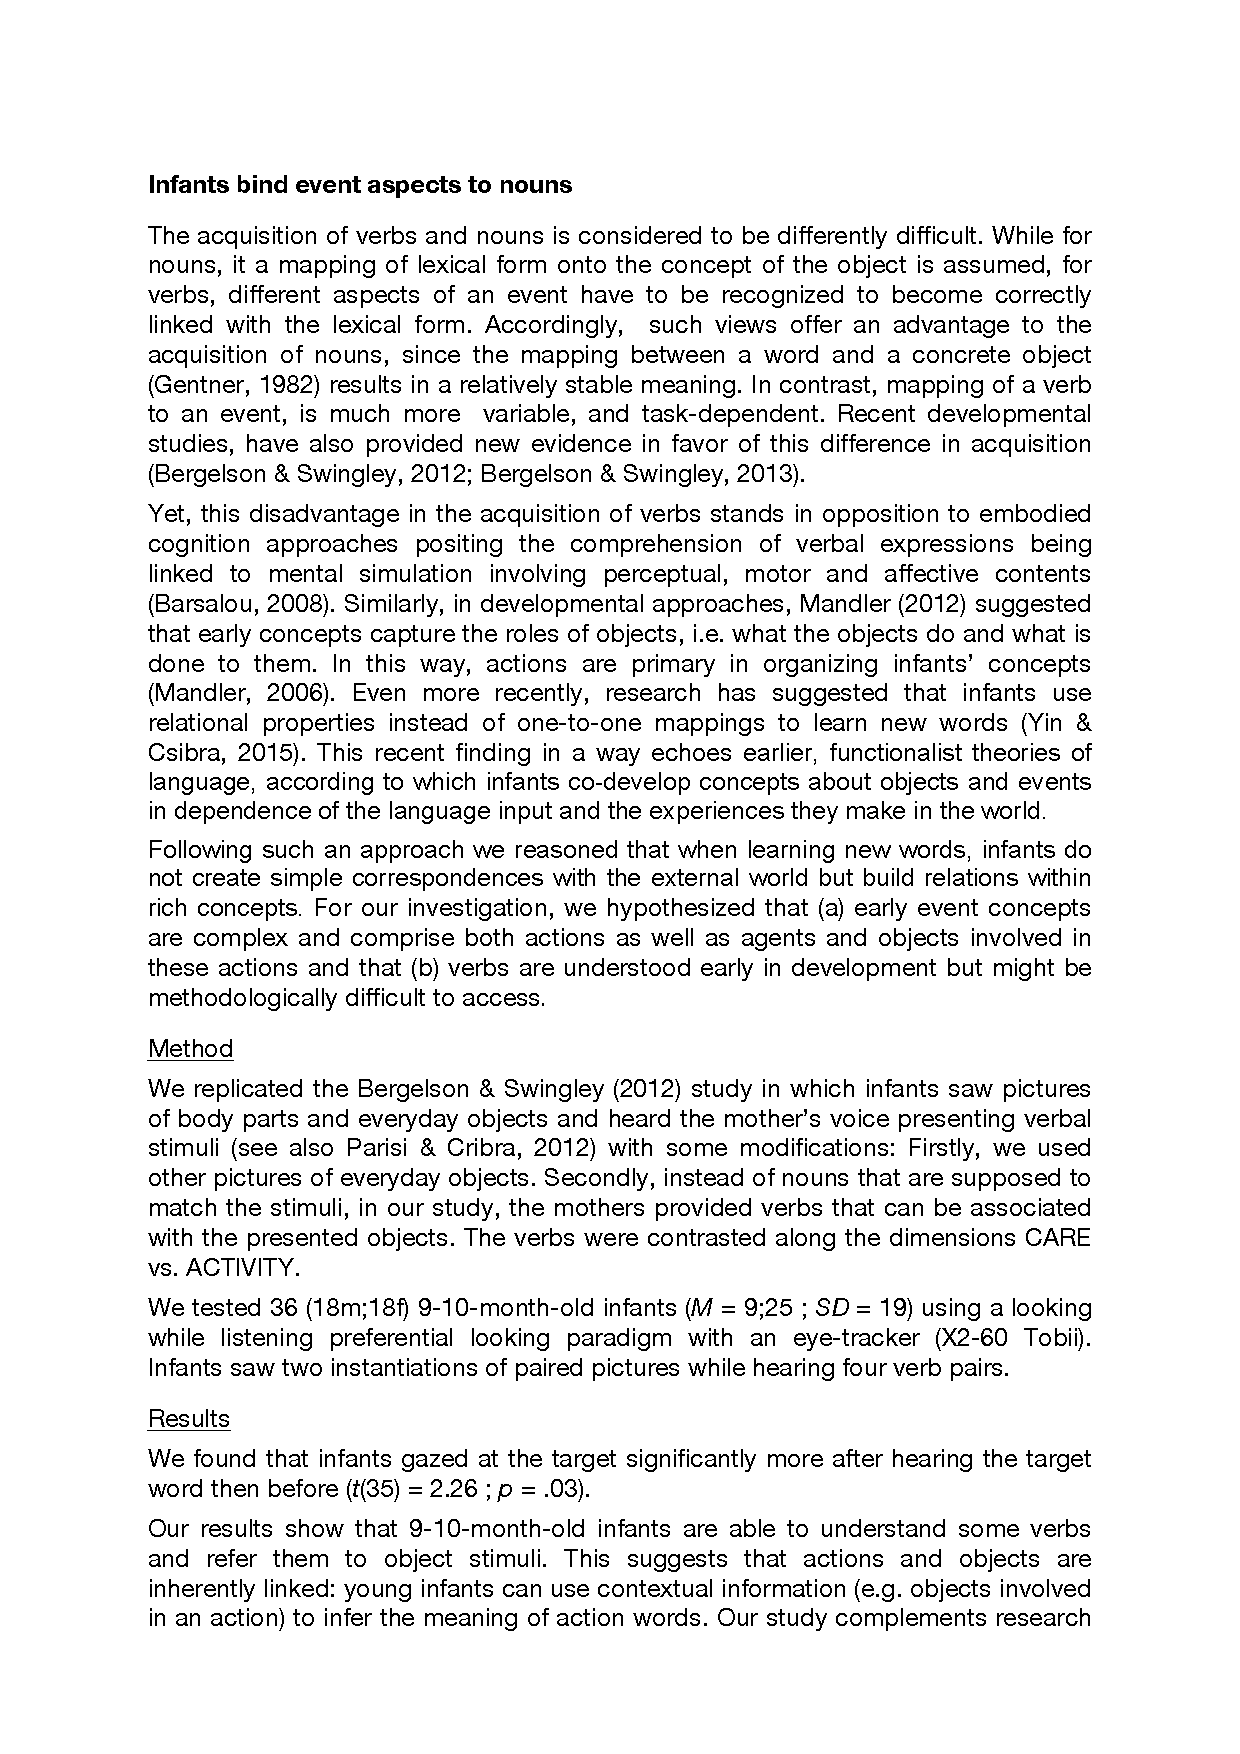
\includepdf[pagecommand={\thispagestyle{plain}}, pages=-]{20_ELC2016_paper_23.pdf}
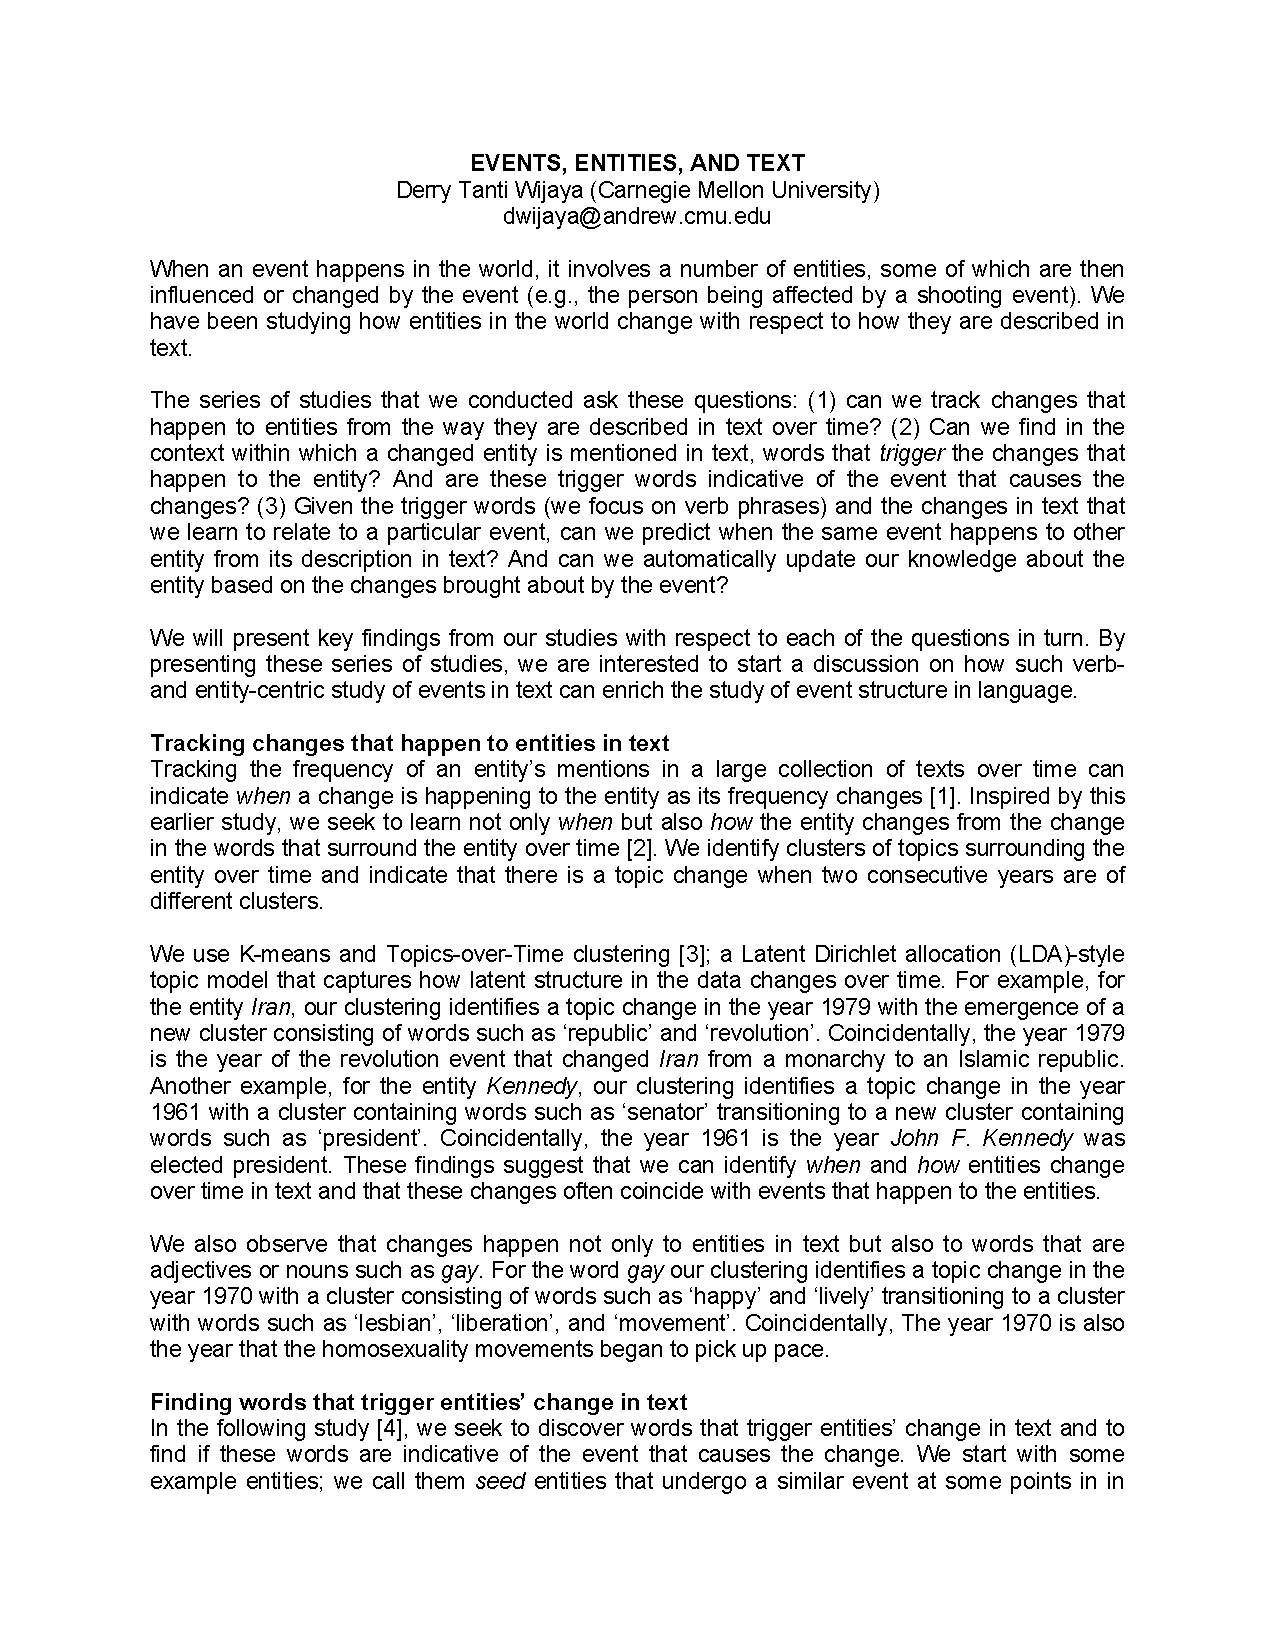
\includepdf[pagecommand={\thispagestyle{plain}}, pages=-]{22_abstract_derry_wijaya.pdf}
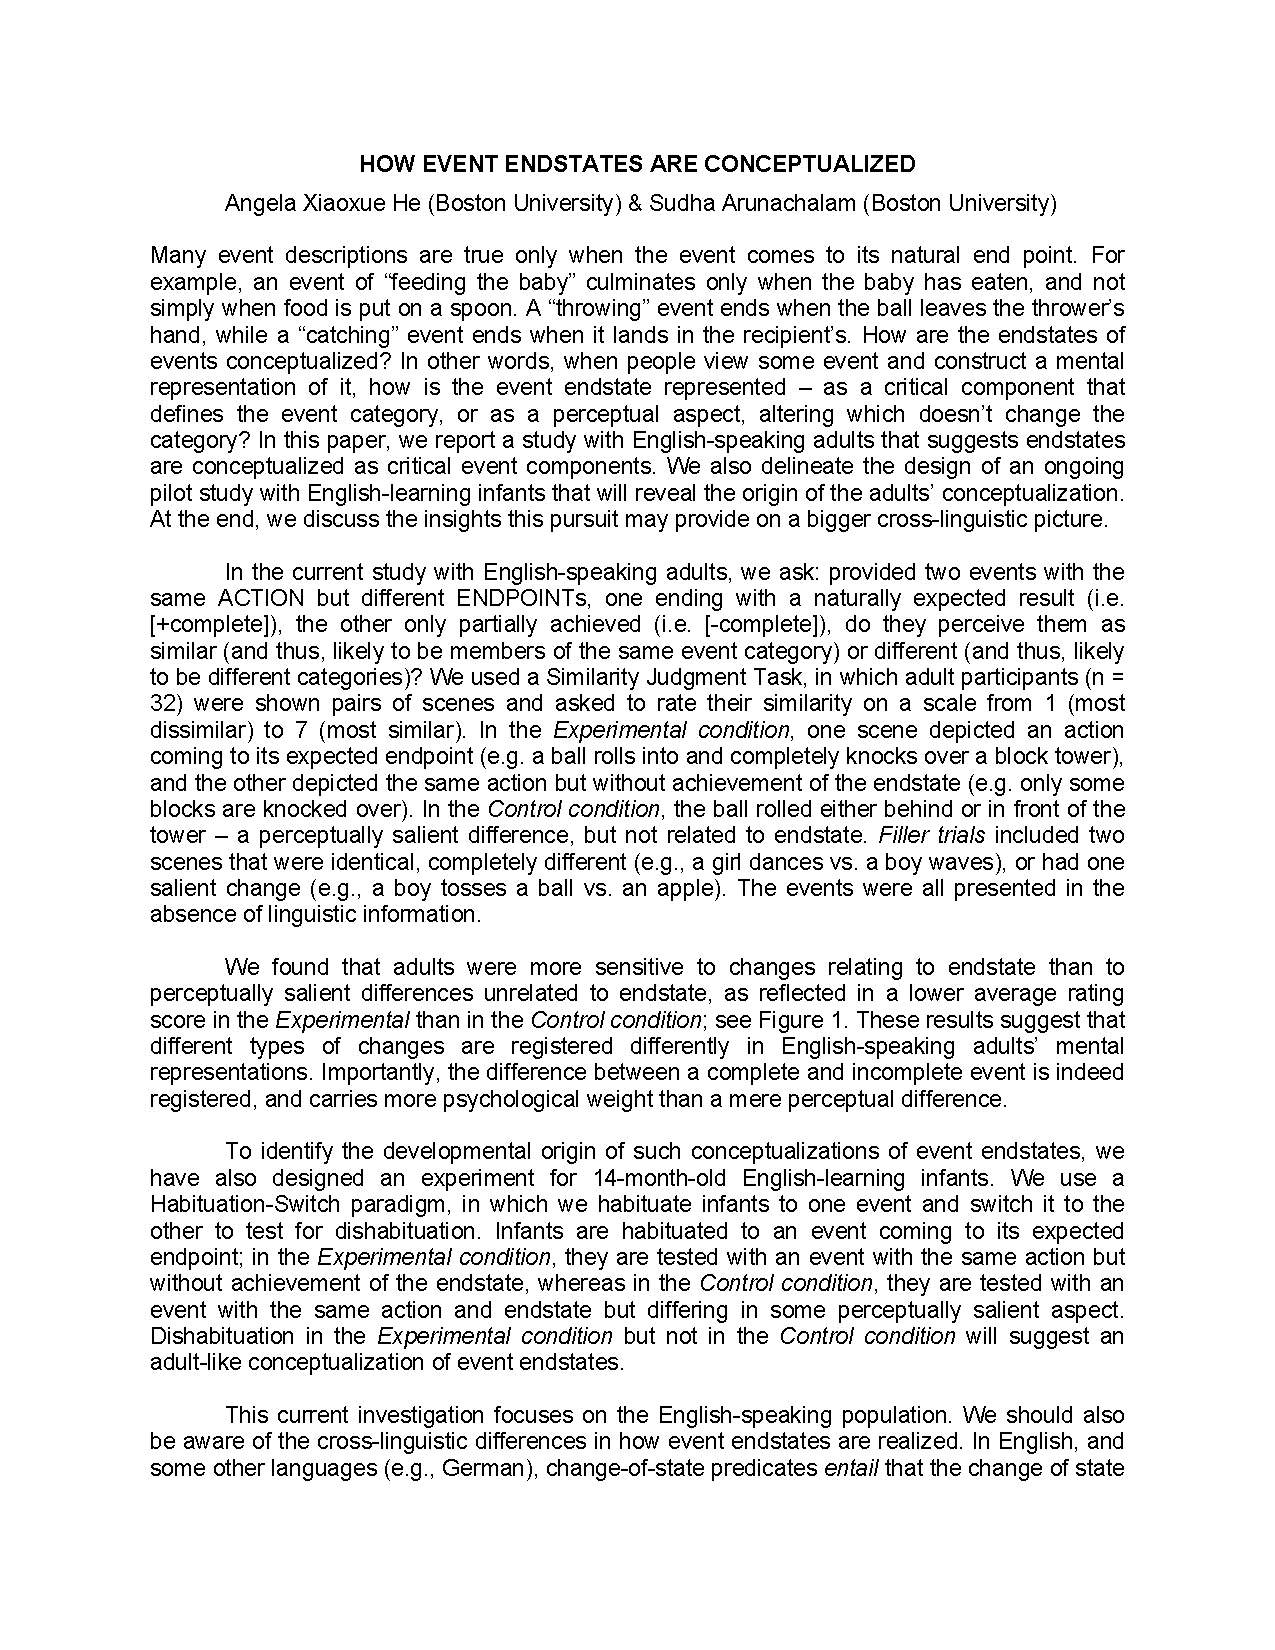
\includepdf[pagecommand={\thispagestyle{plain}}, pages=-]{25_ELC2016-He&Arunachalam.pdf}
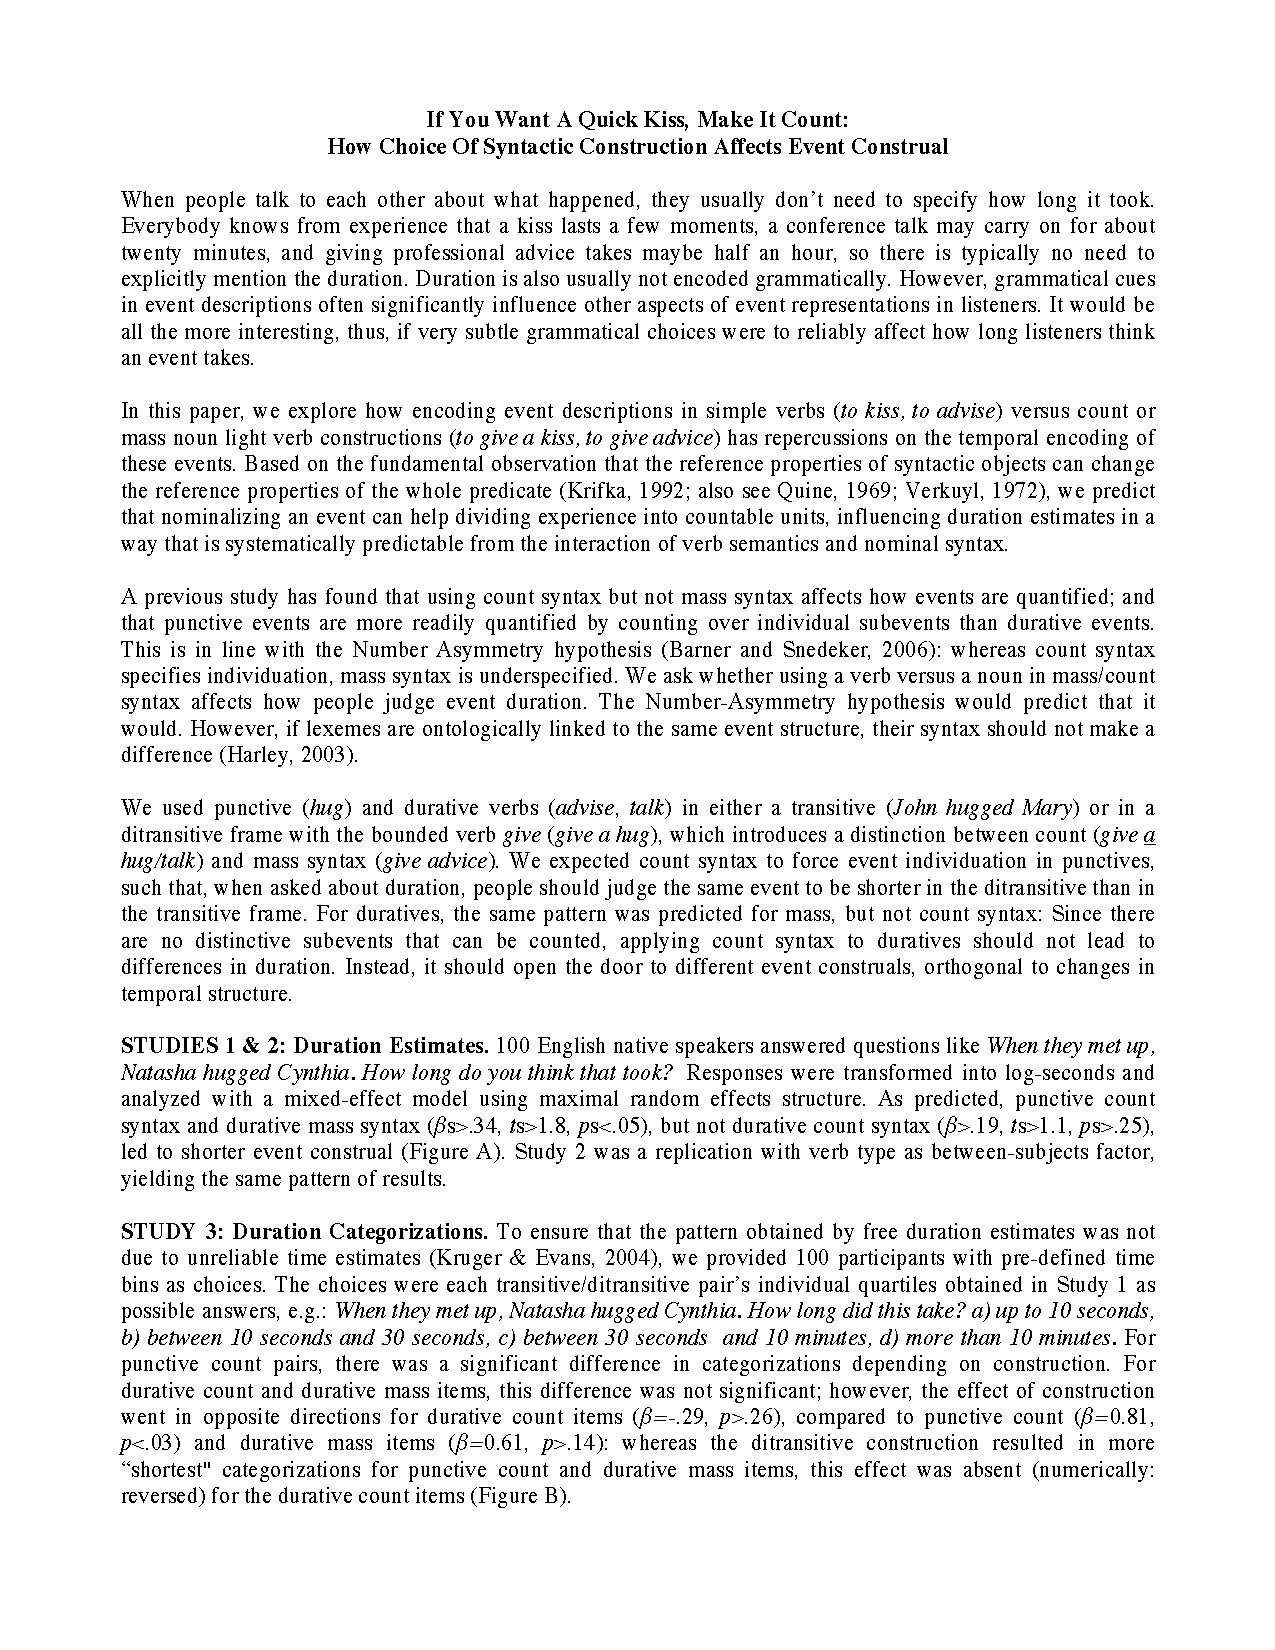
\includepdf[pagecommand={\thispagestyle{plain}}, pages=-]{26_MassCountTime_WittenbergLevy.pdf}

\end{document}
